\documentclass{article}

\usepackage{coursenotes}

\usetikzlibrary{shapes,arrows}
\tikzset{%
pics/.cd,
nodea/.style args={#1#2#3}{
    code={\node[minimum height=2cm] (#3) {\color{#1}#2};
             \draw[thick] (#3.south west) -| (#3.north east)--(#3.north west);
    }
},
%pics/.cd,
nodeb/.style args={#1#2#3}{
    code={\node[minimum height=2cm] (#3) {\color{#1}#2};
             \draw[thick] (#3.south east) -| (#3.north west)--(#3.north east);
    }
},
%pics/.cd,
nodec/.style args={#1#2#3}{
    code={\node[draw,thick,shape=circle,inner sep=1cm] (#3) {\color{#1}#2};
    }
},
}

\set{AuthorName}{TC Fraser}
\set{Email}{tcfraser@tcfraser.com}
\set{Website}{www.tcfraser.com}
\set{ClassName}{Statistical Mechanics}
\set{School}{University of Waterloo}
\set{CourseCode}{Phys 359}
\set{InstructorName}{Michel Gingras}
\set{Term}{Winter 2016}

\begin{document}

\titlePage

\tableOfContents

\disclaimer

\section{Introduction}

\subsection{What is Statistical Mechanics}

Statistical Mechanics is the area of Physics interested in systems with a large number of degrees of freedom $n$. Note that these variables can be interacting or not. \\

There are two distinct class of Statistical Mechanics: equilibrium and non-equilibrium. \\

The Statistical part of Statistical Mechanics implies that it is inherently a study of probabilities and probability distributions. These laws must still remain fully consistent with physical laws. \\

Typically, systems are analyzed on a microscopic level. For a system of particles with charges $\bc{q_i}$ and their positions $\bc{\vec{r}_i}$, the dynamics are governed by the forces acting on each particle,

\[ \vec{F}_i = m_i \vec{a}_i = \sum_{i\neq j} \f{q_iq_j}{4\pi\ep_0} \f{1}{\abs{\vec{r}_{ij}}^2} \]

But does labeling the particles really matter? For the case of $N \ar \infty$, the global phenomenology is of interest.

\subsection{History}

\begin{itemize}
        \item [1738] Daniel Bernoulli
        \begin{itemize}
                \item molecules moving in container, they collide with one another
                \item collisions with walls explains pressure
        \end{itemize}
        \item [$~$1850] Gay Lussac, Joule, Thomson (Lord Kelvin), Carnot
        \item [1859] James Clerk Maxwell
        \begin{itemize}
                \item $D(\nu) \sim e^{-\f{\nu^2}{2k_B T}}$
        \end{itemize}
        \item [1884] Josiash Willard Gibbs
        \begin{itemize}
                \item ensemble averaging
        \end{itemize}
        \item [$~$1900] Planck, Einstein, Bose, Pauli, Fermi, Dirac
        \item [Today] Frontier is in non-equilibrium Statistical Mechanics
        \begin{itemize}
                \item cold atoms
                \item biology
                \item quantum information
        \end{itemize}
\end{itemize}

\section{Foundations}

\subsection{Essence of Statistical Mechanics}

\heading{Laws of Thermodynamics}

\begin{tabular}{|c|c|}
        \hline
        Pros & Cons \\
        \hline
        \tabitem great because they are totally general &
        \tabitem does not tell us how to compute anything \\
        \tabitem relationship's (Maxwell's relations) between $c_p, c_v, \al, \kappa$ &
        \tabitem does not tell us what entropy is \\
        \hline
\end{tabular} \\

The \nth{2} law of Thermodynamics reveals $\dif U = \indif Q - \indif W$ where $\indif Q = T \dif S$. \\

But what is $S$ and what does it \textbf{physically} mean? Boltzmann reveals the relation:

\[ S = k_B \ln (\Om) \]

Which we will come back to.

\subsection{Postulate of Statistical Mechanics}

There is only one postulate of Statistical Mechanics:
\begin{displayquote}
        \textit{For an isolated system in equilibrium, all microstates accessible to the system are equally probable.}
\end{displayquote}

In order to digest this postulate, we will require some definitions.

\heading{Definitions}

\begin{itemize}
        \item system
        \begin{itemize}
                \item part of the universe we care about
                \item only weakly coupled to the rest of the universe
                \item the dynamics/mechanics are dominated by the internal degrees of freedom and forces
        \end{itemize}
        \item isolated
        \begin{itemize}
                \item idealization
                \item eliminates all external influences; no force, no energy/heat flux and no particle flux
                \item quantities such as the energy, number of particles and volume assumed constant forever $\dif U, \dif N, \dif V = 0$
        \end{itemize}
        \item equilibrium
        \begin{itemize}
                \item everything is no-longer changing
        \end{itemize}
        \item microstate
        \begin{itemize}
                \item a complete/total description of everything at the microscopic level $\bc{\vec{r}_i, \vec{p}_i}$ for each $i$
        \end{itemize}
        \item macrostate
        \begin{itemize}
                \item a description at the macroscopic level in accordance with the external constraints
                \item $U, P, T, \bar{M}$
        \end{itemize}
        \item equally probable
        \begin{itemize}
                \item we are dealing with probabilities and statistics
                \item microstates are somehow describing probabilistically the properties at the macroscopic level
        \end{itemize}
        \item accessible
        \begin{itemize}
                \item consistency with the macroscopic constraints imposed by the conservation laws (fixed energy, fixed number of particles)
        \end{itemize}
\end{itemize}

\heading{Postulate Follow-up}

\begin{displayquote}
        \textit{We assume that the observed/realized macrostate is the one with the most microstates.}
\end{displayquote}

\subsection{Perspective from Coin Tossing}

Consider $4$ coins tossed many, many times. What are the microstates describing this system? \\

\newcolumntype{C}{>{\centering\arraybackslash}p{2em}}
\begin{tabular}{|c|CC|CCCC|c|c|}

\hline
Macrostate Label & \multicolumn{2}{c|}{Macrostate} & \multicolumn{4}{c|}{Microstate} & Thermo Probability & True Probability \\
{} & $N_H$ & $N_T$ & A & B & C & D & {} & {} \\
\hline
1 & 4 & 0 & H & H & H & H & 1 & $1/16$ \\
\hline
2 & 3 & 1 & H & H & H & T & 4 & $4/16$ \\
    &   &   & H & H & T & H &   & $    $ \\
    &   &   & H & T & H & H &   & $    $ \\
    &   &   & T & H & H & H &   & $    $ \\
\hline
3 & 2 & 2 & H & H & T & T & 6 & $6/16$ \\
    &   &   & H & T & T & H &   & $    $ \\
    &   &   & T & T & H & H &   & $    $ \\
    &   &   & T & H & H & T &   & $    $ \\
    &   &   & H & T & H & T &   & $    $ \\
    &   &   & T & H & T & H &   & $    $ \\
\hline
4 & 1 & 3 & T & T & T & H & 4 & $4/16$ \\
    &   &   & T & T & H & T &   & $    $ \\
    &   &   & T & H & T & T &   & $    $ \\
    &   &   & H & T & T & T &   & $    $ \\
\hline
5 & 0 & 4 & T & T & T & T & 1 & $1/16$ \\
\hline
\end{tabular}

\vspace{0.1in}

We note that the most probable macrostate $3$ is the one with the most microstates $6$. \\

How do we deal with very large $N, N_H, N_T$ in order to locate the most likely macrostate? First likes get a general expression for $\Om$ were $\Om$ is the number of microstates. Since $N = N_H + N_T$ and $N$ is considered fixed, there is only one free parameter $N_H$ (taken by choice). Thus $\Om$ can be considered a function of $N_H$ and nothing else. \\

Recall from probability that the form for $\Om$ is given by,

\[ \Om = \f{N!}{N_H!\br{N - N_H}!} \]

The most likely macrostate is given when $\Om$ (the number of microstates) is maximized. This means that we are interested in finding values of $N_H$, namely $N_H^*$ where,

\[ \bre{\der{\Om}{N_H}}_{N_H = N_H^*} = 0 \qquad \bre{\dder{\Om}{N_H}}_{N_H = N_H^*} > 0 \]

In order to do this, we will need to explore some mathematics ideas.

\subsection{Stirlings Formula and Gaussian Integrals}

Consider the integral,

\[ I = \intl_0^\inf x^N e^{-x} \dx \]

This can be evaluated using integration by parts,

\[ I = N \intl_0^\inf x^{N-1} e^{-x} \dx = \cdots = N! \numberthis \label{eq:intbypartsNtimes}\]

\subsubsection{Differentiation Trick}

However, integration by parts $N$ times on \eqref{eq:intbypartsNtimes} is annoying. There is a nice trick. Notice that,

\[ \intl_0^\inf e^{-ax} \dx = \bre{-\f1a e^{-ax}}_0^\inf = \f1a \numberthis \label{eq:tricka} \]

One can treat $a$ as a \textit{dummy} variable, and examine \eqref{eq:tricka}'s derivative with respect to $a$,

\[ \pder{}{a} \intl_0^\inf e^{-ax} \dx = \intl_0^\inf \pder{}{a} e^{-ax} \dx = \intl_0^\inf -x e^{-ax} \dx = \pder{}{a}\br{\f1a} = -\f{1}{a^2}\]

The reason for doing this is to simplify the process of \eqref{eq:intbypartsNtimes}. \\

If one explores the $N\tsp{th}$ derivative of \eqref{eq:tricka} with respect to $a$, you will derive the expression,

\[ \bs{\br{-1}^N \pderk{N}{}{a} \intl_0^\inf e^{-ax} \dx}_{a=1} = N! \numberthis \label{eq:trick} \]

The $\br{-1}^N$ term is a result of the alternating sign induced by bringing down a $-x$ each time you take a derivative. \\

\subsubsection{Stirling's Formula}
\label{sec:stirling}

Looking back at the integral \eqref{eq:intbypartsNtimes},

\[ \intl_0^\inf x^N e^{-x} \dx = N! \numberthis \label{eq:stirlingstart}\]

How can we approximate $N!$ using the left had side of \eqref{eq:stirlingstart}? To derive Stirling's Formula, we need to make a change of variables $x = N + \sqrt{N} y$. Substituting into \eqref{eq:stirlingstart} gives,

\[ N! = \intl_0^\inf \sqrt{N} e^{-N} e^{N\ln\br{N+\sqrt{N}y}} e^{-\sqrt{N}y}\dy \]

The approximation begins by expanding the logarithm for large $N$,

\[ \ln\br{N + \sqrt{N}y} = \ln\br{N\bs{1+\f{y}{\sqrt{N}}}} = \ln\br{N} + \ln\br{1+\f{y}{\sqrt{N}}} \]

Take $\ep = \f{y}{\sqrt{N}} << 1$ and apply Taylor series,

\[ \ln\br{1+\ep} \approx \ep - \f{\ep^2}{2} \]

Thus,

\[ N! \approx \sqrt{N}e^{-N}N^N\intl_{-\sqrt{N}}^\inf e^{-\f{y^2}{2}}\dy \]

The lower bound can be approximated as $\inf$ since $N$ is so large,

\[ N! \approx \sqrt{N}e^{-N}N^N\intl_{-\inf}^\inf e^{-\f{y^2}{2}}\dy \]

Notice the remaining integral term. It is called the \textit{Gaussian Integral} and has solution (see \nameref{sec:gaussianintegrals}),

\[ \intl_{-\inf}^\inf e^{-\f{y^2}{2}}\dy = \sqrt{\f{\pi}{a}} \numberthis \label{eq:gaussian} \]

Thus letting $a = 1/2$,

\[ N! \approx \sqrt{2\pi N}e^{-N}N^N \numberthis \label{eq:stirlinglong} \]

Equation \eqref{eq:stirlinglong} is known as \textit{Stirling's Formula}. However, there is a much more useful form of Stirling's Formula. It is obtained by taking the logarithm of both sides,

\[ \ln\br{N!} \approx \br{N+\f12}\ln\br{N} - \br{N - \untext{\f12 \ln\br{2\pi}}{small compared to large $N$}}  \]
\[ \ln\br{N!} \approx N\ln N - N \numberthis \label{eq:stirling} \]

Note that the remaining $N$ is not dropped. This is because for $N \sim 10^{23}$, $N\ln N - N$ and $N\ln N$ differ by about $2\%$. \\

Now we can apply this to the problem of maximizing $\Om$ (which is equivalent to maximizing $\ln\Om$) because the logarithm is monotonically increasing.

\[ 0 = \pder{\ln\Om}{N_H} =\pder{}{N_H} \bs{\ln\br{\f{N!}{N_H!\br{N - N_H}!}}} \]

Through some manipulation, and applying \eqref{eq:stirling}, one obtains the expected result,

\[ N_H = \f{N}{2} \]

\subsubsection{Gaussian Integrals} \label{sec:gaussianintegrals}

Before continuing, we should take a moment to explore how \eqref{eq:gaussian} is solved. Let,

\[ I_x = \intl_{-\inf}^\inf e^{-ax^2}\dx \]

Here comes the trick. Multiply $I_x$ by itself and switch from rectangular coordinates to polar coordinates,

\[ I_xI_y = \intl_{-\inf}^\inf e^{-ax^2}\dx\intl_{-\inf}^\inf e^{-ay^2}\dy \]
\[ I^2 = \intl_{-\inf}^\inf\intl_{-\inf}^\inf e^{-a\br{x^2+y^2}}\dx\dy\]

Where we take $\R^2 (x, y) \mapsto \R^2 (r, \phi)$

\[ I^2 = \intl_{0}^{2\pi} \intl_{0}^\inf re^{-ar^2}\dif r\dif\phi\]

Which reveals that $I^2 = \pi/a$. Thus,

\[ I = \sqrt{\f{\pi}{a}} \]

\subsection{Connections between Thermodynamics and Statistical Mechanics}

Consider a lattice of $\text{Cu}^{2+}$ atoms. In a lattice the $\text{Cu}^{2+}$ atoms are distinguishable because they have unique locations. Now apply an external magnetic field.

\[ H\tsb{Zeeman} = - \vec{\mu} \cdot \vec{B} \]

Recall that $\vec{u} = g \mu_B \vec{s}$ has units $J/T$ where $T$ is Tesla. Where for an electron,

\[ \mu_B = \f{e\hbar}{2m} = \SI{9e-24}{\joule \tesla^{-1}} \qquad g \approx 2 \]

For $\vec{B} = B \hat{z}$, $H\tsb{Zeeman} = 2\mu_BBs_z \defined b s_z$. The splitting of the two spin states $s_z = \pm 1$ for $B = \SI{1}{\tesla}$ has characteristic temperature of,

\[ \f{H\tsb{Zeeman}}{k_B} = \f{\vep}{k_B} = \f{\SI{10e-23}{\joule}}{\SI{1.4e23}{\joule\kelvin^{-1}}} \approx \SI{0.6}{\kelvin} \]

Now consider $N$ electrons subject to the field $\vec{B}$ where there are $N_+$ spins ``up'' and $N_-$ spins ``down''. This is completely analogous to the coin flipping example. The total energy of the system is given by,

\[ U = - N_- \vep + N_+ \vep \]

Note that $N = N_+ + N_-$ and thus,

\[ \f{U}{N} = \vep - 2 \vep \f{N_-}{N} \]

Constraining $U$ and using the substitution,

\[ \f{N_-}{N} = \f{1-x}{2} \qquad \f{N_+}{N} = \f{1+x}{2}\]

Then the microstate measure is given by,

\[ \Om = \f{N!}{N_+!N_-!} \]

Becomes (after some manipulation as using \eqref{eq:stirling})

\[ \ln\Om = -N\bs{\br{\f{1+x}{2}}\ln\br{\f{1+x}{2}} + \br{\f{1-x}{2}}\ln\br{\f{1-x}{2}}} \]

Now recall that for fixed volume $\dif V = 0$,

\[ \f{1}{T} = \br{\pder{S}{U}}_V \]

But since $U$ depends only on $x$, we can write,

\[ \f{1}{T} = \br{\pder{S}{x}}\br{\pder{x}{U}} \]

Thus reveals a slight connection between $S$ the entropy and $\Om$ through $x$ in this example. Further analysis with motivate Boltzmann's equation,

\[ S = k_B \ln\Om + S_0 \]

\subsection{Example of a Physical System with Constraint}

Suppose you have $3$ particles called $A,B,C$ such that each particle can have $\vep_j = j \vep$ where $j = 0, 1, 2, 3, \ldots$. \\

How many microstates are there subject to the constraint that the total energy is $3\vep$? \\

\begin{tabular}{|c|CCCC|CCC|c|c|}

\hline
Macrostate Label & \multicolumn{4}{c|}{Macrostate} & \multicolumn{3}{c|}{Microstate} & Thermo Probability & True Probability \\
{} & $N_0$ & $N_1$ & $N_2$ & $N_3$ & A & B & C & {} & {} \\
\hline
1 & 2 & 0 & 0 & 1 & 0 & 0 & $3\vep$ & 3 & $3/10$ \\
    &   &   &   &   & 0 & $3\vep$ & 0 &   &        \\
    &   &   &   &   & $3\vep$ & 0 & 0 &   &        \\
\hline
2 & 0 & 1 & 1 & 0 & 0 & $\vep$ & $2\vep$ & 6 & $6/10$ \\
    &   &   &   &   & $\vep$ & $2\vep$ & 0 &   &        \\
    &   &   &   &   & $2\vep$ & 0 & $\vep$ &   &        \\
    &   &   &   &   & 0 & $2\vep$ & $\vep$ &   &        \\
    &   &   &   &   & $2\vep$ & $\vep$ & 0 &   &        \\
    &   &   &   &   & $\vep$ & 0 & $2\vep$ &   &        \\
\hline
3 & 0 & 3 & 0 & 0 & $\vep$ & $\vep$ & $\vep$ & 1 & $1/10$ \\
\hline
\end{tabular}

\section{Review of Thermodynamics}

\subsection{Definitions}

Recall Boyle's Law $PV = nRT$.

\begin{itemize}
        \item processes
        \begin{itemize}
                \item constant $T$, isothermal process
                \item constant $P$, isobaric process
                \item constant $V$, isochoric process or isovolumetric process
                \item constant $S$, adiabatic process
                \begin{itemize}
                        \item Comes from greek \textit{diabatos} which means \textit{to go through}
                        \item No heat exchange between system and surroundings
                        \item Can also be an approximation for processes that occur really quickly over a short period of time
                \end{itemize}
        \end{itemize}
        \item processes reversible/irreversible
        \begin{itemize}
                \item reversible process happens over a number of discrete steps and that are each reversible
                \item irreversible processes are like poking a hole in a balloon or a gas expanding in a vacuum
        \end{itemize}
        \item thermodynamic variables $T, P, V, U$ where $U$ is the \textit{total energy}
\end{itemize}

\subsection{Zeroth Law of Thermodynamics}

If systems $A$ and $B$ are in equilibrium with one another and systems $B$ and $C$ are in equilibrium then $A$ is in equilibrium with $C$.

\subsection{Functions of State}

Thermodynamic variables are not independent. They are often related by an equation of state. For example $PV = nRT$ for an ideal gas. Other variables might come into an equation of state. For example $\rho, \mathcal{T}, E$ are all important for the equation of state for a liquid crystal sample. \\

Equations of state with typically look like

\[ f\br{P, V, T} = 0 \]

Another important notion is the notion of \textit{function of state}. A quantity that depends only on the thermodynamic variables of the system and \textit{not it's history}, is called a \textit{function of state}. \\

We will first focus on $U\tsb{total energy}$ first and then $S\tsb{entropy}$ as our functions of state. \\

Mathematically, $G = g\br{x,y}$ where $x,y$ are the thermodynamic variables and $G$ is a function of state analytic everywhere and obeys some properties:

\begin{itemize}
        \item $\dif G = \br{\pder{G}{x}}_y \dx + \br{\pder{G}{y}}_x \dy $
        \item at most values of the thermodynamic variables $g(x,y)$ is ``smooth''.
        \item for example: $\br{\pdder{G}{x}}_y$ or $\br{\pdder{G}{y}}_x$ or $\br{\pder{}{x}\br{\pder{G}{y}}_x}_y$ are all continuous
        \item the order of discontinuities is determined by whether or not the system or substance is undergoing transitions of state or not
\end{itemize}

For functions of state that are analytical everywhere, the order of derivatives is inconsequential.

\[ \br{\pder{}{x}\br{\pder{G}{y}}} = \br{\pder{}{y}\br{\pder{G}{x}}}\]

What can we say about $G$ in cases where

\[ \dif G = \pder{G}{x} \dx + \pder{G}{y} \dy \numberthis \label{eq:dg} \]

in the case of functions of state like $U$, $ \dif U = \indif Q - \indif W  $ and the inexact differentials and how they relate to exact differentials like $\dif V$ and $\dif S$? In particular, when can we integrate $\dif U$?

Answer: equation \eqref{eq:dg} can be integrated in situations where

\[ \br{\pder{}{y}\br{\pder{G}{x}}_y}_x = \br{\pder{}{x}\br{\pder{G}{y}}_x}_y \numberthis \label{eq:exactcond}\]

When equation \eqref{eq:exactcond} is held for a physical system, one can say that $\dif G$ is an \textbf{exact differential}. Review 12,13 in notes on ``Review of Thermodynamics''. \\

The difference in the function $G(x,y)$ between two sufficiently close pairs of points $(x_1, y_1)$ and $(x_2, y_2)$ depends only on the difference in $G(x,y)$ evaluated at those two points.

\[ \Delta G = G(x_2, y_2) - G(x_1, y_1) \]

$\Delta G$ does not depend on the path from point $(x_1, y_1)$ to $(x_1, y_1)$. In practice, one can assign such a function $G$ to the values of the thermodynamic variables at the points $(x,y)$. For example, $U(P,V)$ is such a function of state. It depends only on the description through the thermodynamic variables and not the history. \\

By counter example, heat $Q$ is not a function of state. No one can say, ``that substance has $X$ units of heat in it''.

\subsection{Work}

There are two types of work. One is called \textit{configuration work} and the other is called \textit{dissipative work}. \\

\subsubsection{Configuration Work}

Configuational work is denoted $\indif W$ where the symbol $\indif$ represents that it \textbf{is not} and exact differential.

\[ \indif W = \sum_i y_i \dif x_i \]

where $y_i$ is an intensive variable (not proportional to $N, V$; examples: pressure, surface tension). It can be thought of as a generalized force. Here $\dif x_i$ is the generalized displacement which is an extensive variable.

\subsubsection{Dissipative Work}

Dissipative work can be thought of as ``stirring work''. Examples include a mixer in a liquid or an electrical wire/resistor.

\begin{itemize}
        \item electrical power:
        \begin{itemize}
                \item $P = V \cdot I$
                \item $\dif W\tsb{dis} = P \cdot \dif t = R I^2 \dif t$
        \end{itemize}
\end{itemize}

\subsubsection{Sign Convention}

\[ \indif W > 0 \note{work done by the system} \]
\[ \indif W < 0 \note{work done on the system} \]

Note:

\begin{itemize}
        \item work is \textbf{not} a property of the system
        \item work is \textbf{not} a function of state
        \item integration on a closed loop is not degenerate $\oint \indif W \neq 0$
\end{itemize}

\subsubsection{Abiabatic Work}

Adiabatic work occurs with no heat exchange.

\begin{center}
\begin{tikzpicture}[scale=1.0]
        % Draw axes
        \draw [<->,thick] (0,4) node (yaxis) [above] {$P$}
                |- (5,0) node (xaxis) [right] {$V$};
        \coordinate (f) at (4,1);
        \coordinate (i) at (1,3);
        \node [blue, label={[blue]10:$\indif Q = 0$}] (mid) at (2, 1.5) {};
        \draw [blue, thick, ->] plot [smooth, tension=1] coordinates { (i) (mid) (f)};
        \node [below] (vi) at (1,0) {$V_i$};
        \node [below] (vf) at (4,0) {$V_f$};
        \node [left] (pf) at (0,1) {$P_f$};
        \node [left] (pi) at (0,3) {$P_i$};
        \draw [gray, dashed] (i) -- (vi);
        \draw [gray, dashed] (i) -- (pi);
        \draw [gray, dashed] (f) -- (vf);
        \draw [gray, dashed] (f) -- (pf);
\end{tikzpicture}
\end{center}

Adiabatic work is done between any two equilibrium states and is \textit{independent of path}. One can define a function of state as the total adiabatic work done on a system. Lets define this a the total internal energy of the system.

\[ \dif U = - \dif W\tsb{adiabatic}\]

Note the minus `$-$' sign is due to the fact that the total energy of the system increases when work is done \textbf{on} this system. Along adiabatic paths, there is an exact differential associated with $\indif W$. It is called internal energy $\dif U$.

\subsection{First of Law of Thermodynamics}

\subsubsection{Heat}

In systems such as boiling a pot of water, there is no work performed on the system however the state of the system changes (not boiling to boiling). The mechanism that causes this change of state is heat ($Q$).

\[ \dif U = \indif W + \indif W \numberthis \label{eq:firstlaw} \]

Equation \eqref{eq:firstlaw} is using the following convention:

\begin{align*}
        \indif Q &:< 0 \note{heat flow \textbf{in}} \\
        \indif Q &:> 0 \note{heat flow \textbf{out}} \\
        \indif W &:< 0 \note{work is done \textbf{by} system} \\
        \indif W &:> 0 \note{work is done \textbf{on} system} \\
\end{align*}

\subsubsection{Heat Capacities}

Use the convention that $C$ is the heat capacity (extensive) and $c$ is the specific heat capacity (intensive).

\[ c = \f{C}{n} \]

\[ C \defined \lim_{\Delta T \ar 0} \f{\Delta Q}{\Delta T} \]

Heat capacity $C$ is very important. Measuring $C$ in a metal at low temperatures reveals very important intrinsic properties of the material. Also note that heat capacity is always $C \sim \f1T$ and not some other power than $-1$.

\heading{Relationship Between $c_v, c_p$ for an Ideal Gas}

\[ PV = nRT \]

Using Boyle's law, work with $n = \SI{1}{\mole}$ for convenience. How can we relate $C$ to the properties of the substance? Let us write (noting the `-' convention),

\[ \dif U = \indif Q - \indif W \]

Switch to specific (per mole) quantities,

\[ \dif u = \indif q - \indif w \]

\[ \dif u = \pdert{u}{T}{v} \dif T + \pdert{u}{v}{T} \dif V \]

\[ \indif q = \dif u + \indif w \]
\[ \indif q = \pdert{u}{T}{v} \dif T + \bc{\pdert{u}{v}{T} \dif V + P\dif v} \]

However,

\[ c_v = \lim_{\dif T \ar 0} \f{\indif q}{\dif T} \note{At constant V} \]

Thus,

\[ c_v = \pdert{u}{T}{v} \numberthis \label{eq:heatcapacity} \]

Which gives us,

\[ \indif q = c_v \dif T  + P\dif v \]

Note that this formula uses the fact that,

\[ \pdert{U}{v}{T} = 0 \note{For ideal gas.} \]

Which we will prove momentarily, but can be taken as an experimental fact discovered by Guy-Lussac. Namely $U$ is only a function of $T$ for an ideal gas ($U = U(T)$).

\[ \indif q = c_v \dif T  + P\dif v + \br{ v \dif p  - v\dif p} \]
\[ \indif q = \br{c_v + R} \dif T  - v\dif p \]

Thus,

\[ \lim_{\dif T \ar 0} \bre{\f{\indif q}{\dif T}}_{p=\text{const.}} = c_v + R \]

Thus we can define a new quantity,

\[ c_p \defined \bre{\f{\indif q}{\dif T}}_{p=\text{const.}} = c_v + R \]

For an monoatomic gas ($U = \f32 RT$),

\[ \ga \defined \f{c_p}{c_v} = \f{5}{3} \]

\subsection{Adiabatic Work Continued}

Let us examine an isotherm (red) next to an adiabatic curve (blue),

\begin{center}
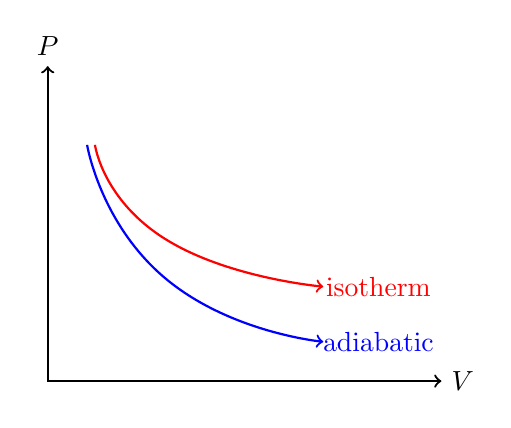
\begin{tikzpicture}[scale=1.0]
        % Draw axes
        \draw [<->,thick] (0,4) node (yaxis) [above] {$P$}
                |- (5,0) node (xaxis) [right] {$V$};
        \draw [blue, thick, ->] plot [smooth, tension=1] coordinates { (0.5,3) (1.5, 1.3) (3.5, 0.5)};
        \draw [red, thick, ->] plot [smooth, tension=1] coordinates { (0.6,3) (1.5, 1.8) (3.5, 1.2)};
        \node [blue] (adiabatic) at (4.2, 0.5) {adiabatic};
        \node [red] (isotherm) at (4.2, 1.2) {isotherm};
\end{tikzpicture}
\end{center}

\begin{align*}
        \indif q &= c_v \dif T + P \dif v \\
        \indif q &= c_P \dif T - v \dif P
\end{align*}

And let's set $\indif q = 0$ (adiabatic),

\[ c_v \dif T + P \dif v = c_P \dif T = v \dif P \]

Which gives,

\[ \f{\dif P}{P} = - \ga \f{\dif v}{v} \note{Using $\ga = c_P/c_v$} \]

Or integrating along a curve,

\[ \intl_1^2 \f{\dif P}{P} = - \intl_1^2 \ga \f{\dif v}{v} \]
\[ \ln\br{\f{P_2}{P_1}} = - \ga \ln\br{\f{v_2}{v_1}} \]

Which gives the relationship,

\[ P_1V_1^\ga = P_2V_2^\ga \]

Which holds true along an adiabatic curve. However, $PV = RT$. Thus using the expression $\dif U = - P \dif V |\tsb{adiabatic}$ gives the result,

\[ W = \bc{\f{P_2V_2 - P_1V_1}{1-\ga}}_{\ga > 1} \]

\subsubsection{Gay-Lussac Experiment}
\label{sec:guylussac}

For an ideal gas,

\[ \pdert{U}{V}{T} = 0 \]

\[ \indif Q = \pdert{U}{T}{V} \dif T + \bc{\pdert{U}{V}{T} + P}\dif V \]

\[ \f{\indif Q}{T} = \f{1}{T}\pdert{U}{T}{V} \dif T + \f{1}{T}\bc{\pdert{U}{V}{T} + P}\dif V \]

Employ an integrating factor for the inexact differentials. It will take us from and inexact differential to an exact differential.

\heading{Math Interlude}

\[ \indif G = A(x,y)\dx + B(x,y)\dy \]

Multiply $G$ by $\mu(x,y)$ and unknown function of $x$ and $y$,

\[ \dif \ti{G} = \mu \cdot \indif G\]

Thus,

\[ \dif \ti{G} = \mu A \dx + \mu B \dy \]

Making,

\[ \pder{\br{\mu A}}{y} = \pder{\br{\mu B}}{x} \numberthis \label{eq:intfact} \]

\heading{Example}

\[ \dif G = \sin(y) \dx + \cos(y) \dy \]
\[ \dif \ti{G} = \mu\sin(y) \dx + \mu\cos(y) \dy \]

Let us look for a $\mu$ such that $\mu(x,y) = \mu(x)$ and plugging into equation \eqref{eq:intfact},

\[ \pder{\br{\mu \sin(y)}}{y} = \pder{\br{\mu \cos(y)}}{x} \]
\[ \mu(x)\cos(y) = \der{\mu}{x}\cos(y) + \mu \der{\cos{y}}{x} \]
\[ \mu(x)\cancel{\cos(y)} = \der{\mu}{x}\cancel{\cos(y)} + \mu \cancelto{0}{\der{\cos{y}}{x}} \]

Thus,
\[ \mu(x) = \der{u}{x} \]
Which gives,
\[ \mu(x) = e^x \]

The purpose of introducing the notion of an integrating factor is to reveal that although $\indif Q$ is an inexact differential, we can introduce an integrating factor $\f1T$ that makes the quantity $\f{\indif Q}{T}$ an \textbf{exact} differential. This quantity is somehow more important that $Q$ as it describes a property of the system. We will see that this quantity is the motivation for entropy. Let us examine this,

\[ \f{\indif Q}{T} = \underbrace{\f{1}{T}\pdert{U}{T}{V}}_{A} \dif T + \underbrace{\f{1}{T}\bc{\pdert{U}{V}{T} + P}}_{B}\dif V \]

And thus,

\[ \pder{A}{V} = \pder{B}{T} \]

Gives,

\[ \pder{A}{V} = \pder{}{V}\bc{\f1T \pder{U}{T}} = \f1T \f{\partial^2 U}{\partial V \partial T} \]
\[ \pder{B}{T} = \pder{}{T}\bc{\f1T \br{\pder{U}{V} + P}} = -\f{1}{T^2} \br{\pder{U}{V} + P} + \f1T \f{\partial^2 U}{\partial T \partial V} + \f1T \pder{P}{T} \]

Equating these two expressions (noticing that $\f{\partial^2 U}{\partial T \partial V} = \f{\partial^2 U}{\partial V \partial T}$ and that $PV = RT \implies \f{P}{T^2} = \f{R}{TV}$),

\[ \f1T \f{\partial^2 U}{\partial V \partial T} = -\f{1}{T^2} \br{\pder{U}{V} + P} + \f1T \f{\partial^2 U}{\partial T \partial V} + \f1T \pder{P}{T} \]
\[ \cancel{\f1T \f{\partial^2 U}{\partial V \partial T}} = -\f{1}{T^2} \br{\pder{U}{V} + P} + \cancel{\f1T \f{\partial^2 U}{\partial T \partial V}} + \f1T \pder{P}{T} \]
\[ 0 = -\f{1}{T^2} \br{\pder{U}{V} + P} + \f1T \pder{P}{T} \]
\[ \f{1}{T^2} \br{\pder{U}{V} + P} = \f1T \pder{P}{T} \]
\[ \f{1}{T^2} \pder{U}{V} + \f{P}{T^2} = \f1T \pder{P}{T} \]
\[ \f{1}{T^2} \pder{U}{V} + \cancel{\f{R}{TV}} = \cancel{\f{R}{TV}} \]

Therefore Gay-Lussac was destined to find this relationship through experiment:
\[ \pder{U}{V} = 0 \]

\subsubsection{Joule-Thomson(Kelvin) Experiment}

Using $\f{1}{T}$ as the integrating factor, one can go through a similar derivation as in section \ref{sec:guylussac} to understand that the quantity $S$ is a state function of a system with,

\[ \dif S \defined \f{\indif Q}{T}  \]

\subsubsection{Summary of First Law}

In summary, the first law of thermodynamics is really just conservation of energy with expression,

\[ \dif U = \indif Q - \indif W \]

\subsection{Second Law of Thermodynamics}

Physical laws on the microscopic scale always are found to have an inherent time-reversal symmetry. The physics behaves the same running forward in time and backward in time. However, a semi-paradox of real-world phenomenology seems to suggest that there are some processes can not occur moving backward in time. They still satisfy the conservation of energy, but there is another law that governs these macroscopic phenomena.

\subsubsection{Heat Engines}

Imagine a an engine $E$ that runs from temperature $T_2$ to $T_1$ (two heat baths), where it extracts heat $Q_2$ and disposes heat $Q_1$ and does some work $W$.

\begin{center}
\begin{tikzpicture}[scale=2]
        \pic at (0,0) {nodea={red}{$T_H$}{L}};
        \pic at (2,0) {nodec={black}{}{C}};
        \pic at (4,0) {nodeb={blue}{$T_C$}{R}};
        \draw[->,>=latex](L)--node[midway,above]{$Q_2$}(C);
        \draw[->,>=latex](C)--node[midway,above]{$Q_1$} (R);
        \draw[->,>=latex](C)--node[midway,left]{$W$} ++(0,-2cm);
\end{tikzpicture}
\end{center}

The efficiency of the engine is defined as,

\[ \eta \defined \f{\text{output}}{\text{input}} = \f{W}{Q_2} \]

Note that on a cyclic process $\De U = 0$ since $U$ is a function of state. However it is also equal to,

\[ \De U = \br{Q_1 + Q_2} - W \]

Therefore typically the efficiency is given by,

\[ \eta = 1 + \f{Q_1}{Q_2} \]

\begin{itemize}
    \item $Q_2$ : injected into engine $E$ and is $>0$
    \item $Q_1$ : extracted from engine $E$ and is $<0$
\end{itemize}

This can be re-written as,

\[ \eta = 1 + \f{Q_1}{-\abs{Q_2}} = 1 - \f{\abs{Q_1}}{\abs{Q_2}} \]

\subsubsection{Carnot Cycle/Engine}

It can be shown that no engine is more efficient than a Carnot engine. Upon considering this, one can use entropy to expose the Second Law of Thermodynamics and the natural ``arrow of time''.

\begin{center}
\begin{tikzpicture}[
    scale=1.0,
    decoration={post length=0.1mm, pre length=0.1mm, markings, mark=at position 0.5 with {\arrow{>}}}
]
        % Draw axes
        \coordinate (nya) at (0, 0);
        \coordinate (pya) at (0, 4);
        \coordinate (nxa) at (0, 0);
        \coordinate (pxa) at (5, 0);
        \node [above] (lpya) at (pya) {$P$};
        \node [right] (lpxa) at (pxa) {$V$};
        \coordinate (a) at (1.1, 3);
        \coordinate (b) at (3.2, 2.2);
        \coordinate (c) at (4, 1);
        \coordinate (d) at (2, 1.5);
        \draw [->, thick] (nya) -- (pya);
        \draw [->, thick] (nxa) -- (pxa);
        \draw [postaction={decorate}, thick] (a) -- (b);
        \draw [postaction={decorate}, thick] (b) -- (c);
        \draw [postaction={decorate}, thick] (c) -- (d);
        \draw [postaction={decorate}, thick] (d) -- (a);
        \node [above left] (la) at (a) {$a$};
        \node [above right] (lb) at (b) {$b$};
        \node [below] (lc) at (c) {$c$};
        \node [below left] (ld) at (d) {$d$};
\end{tikzpicture}
\end{center}

\begin{center}
\begin{tabular}{c|c|c|c}
$ab$ & isotherm ($T_2$) & $Q_2 > 0$ & $W^{ab} > 0$\\
\hline
$bc$ & adiabat & $Q = 0$ & $W^{bc} > 0$\\
\hline
$cd$ & isotherm ($T_1$) & $Q_1 < 0$ & $W^{cd} < 0$\\
\hline
$da$ & adiabat & $Q = 0$ & $W^{da} < 0$\\
\end{tabular}
\end{center}

The total work is given by,

\[ W\tsb{tot} = W^{ab} + W^{bc} + W^{cd} + W^{da} \]

1) First the isotherms:

\[ W \sim \int P\dif V \note{Use $PV = RT$ (1 mole)}\]
\[ W = \intl_1^2 \f{RT}{V} \dif V = RT \ln\br{\f{V_2}{V_1}} \]
\begin{center}
\begin{tabular}{c|c|c}
$ab$ & $RT_2 \ln\br{\f{V_b}{V_a}} > 0$ & $\implies Q_2$\\
\hline
$cd$ & $RT_1 \ln\br{\f{V_d}{V_c}} < 0$ & $\implies Q_1$\\
\end{tabular}
\end{center}
This is to be expected because we are on isotherms and $\Delta U = 0$. \\

2) Second the adiabats:

Along an adiabat,

\[ PV^{\ga} = \text{const.}\]
\[ P_1V_1^{\ga} = P_2V_2^{\ga} \]

Furthermore, relating this to $PV = RT$,

\[ \f{RT_1}{V_1} V_1^{\ga} = \f{RT_2}{V_2} V_2^{\ga} \]
\[ T_1 V_1^{\ga-1} = T_2 V_2^{\ga-1} \]

Applying this to our diagram,

\[ T_2 V_b^{\ga-1} = T_1 V_c^{\ga-1} \quad \text{and} \quad T_1 V_d^{\ga-1} = T_2 V_a^{\ga-1} \]

Which after rearrangement yields a constraint for the volumes,

\[ \f{V_b}{V_a} = \f{V_c}{V_d} \]

Therefore,

\[ \eta\tsb{Carnot} = \eta_C = 1 + \f{Q_1}{Q_2} \]
\[ \eta_C = 1 + \f{RT_1\ln\br{V_d/V_c}}{RT_2\ln\br{V_b/V_a}} = 1 - \f{T_1}{T_2}\f{\ln\br{V_c/V_d}}{\ln\br{V_b/V_c}} \]
\[ \eta_C = 1 - \f{T_1}{T_2} \]

\subsubsection{Second Law Statements}

\begin{enumerate}
    \item \textbf{Clausius:} You can not build a machine or engine operating in a cycle can be constructed whose sole effect is to transfer heat from a cold to hot.
    \item \textbf{Kelvin-Planck:} It is impossible to construct a device whose sole effect is to produce work by only absorbing heat from a single reservoir. Two reservoirs are needed.
\end{enumerate}

Now let us use Clausius statement to prove Carnot's theorem as per the Carnot Engine; the most efficient engine is a Carnot engine.

\heading{Example}

Suppose we have an engine $E$ that extracts heat from a hot $T_2$ reservoir $Q_2 = \SI{100}{cal}$, performs $W = \SI{20}{cal}$ of work and then dumps the remaining $Q_1 = \SI{80}{cal}$ calories of heat into a cold reservoir $T_1$. This is our Carnot engine.

\[ \eta_C = \f{W}{Q_2} = \f{20}{100} = 20\% \]

Now suppose we had a better engine with $\eta_y > \eta_C$. Namely, this new engine has specs $Q_2 = \SI{100}{cal}, W = \SI{40}{cal}, Q_1 = \SI{60}{cal}$.

\[ \eta_y = \f{W}{Q_2} = \f{40}{100} = 40\% \]

Now to prove is can not be the case, let us take our Carnot engine and reverse it's processes (making it a fridge), and doubling it's size. Therefore this Carnot fridge will require $\SI{40}{cal}$ to run. This can be supplied by our ``better'' engine. Therefore, this combined engine has the net effect of absorbing $\SI{100}{cal}$ from a cold reservoir at $T_1$ and injecting $\SI{100}{cal}$ into a hot reservoir at temperature $T_2$, \textbf{with no other effect.} This violates the Clausius hypothesis.

\heading{Corollary}

All engines operating reversibly between two temperatures $T_1$ and $T_2$ have the same efficiency. In other words, the presence of any irreversible process degrades the efficiency.

\[ \eta\tsb{irreversible} < \eta\tsb{Carnot} \numberthis \label{eq:irreversiblecarnot}\]

\subsubsection{Entropy}

We have found that,

\[ \eta_C = 1 + \f{Q_1}{Q_2} = 1 - \f{T_1}{T_2} \]

Or equivalently,

\[ \f{Q_1}{T_1} + \f{Q_2}{T_2} = 0 \]

For a single Carnot engine, the sum of heat at step $n$ over the temperature at step $n$ has sum,

\[  \sum_{n=1}^{k} \f{Q_n}{T_n} = 0 \numberthis \label{eq:revcarnot}\]

Which gives that $\De Q / T$ over the whole cycle is zero. Taking the limit as $k \ar \inf$, it suggests that the quantity $\indif Q / T$ is an exact differential. Introduce the label of entropy,

\[ \dif S = \f{\indif Q}{T} \quad \text{with} \quad \oint \dif S\tsb{rev} = 0  \]

As you can see, considering a Carnot engine also suggests the presence of a quantity $S$ call entropy. Just as before, $S$ is a state function. \\

How can we compute entropy? \\

\heading{Example (Constant Volume)}

Let's consider heat injected at constant volume, and attempt to calculate $\De S$.

\[ \De U = \De Q - \De W \note{At constant volume, $\De W = 0$} \]

But we also have $\De Q = C_v \De T$ where $C_v$ is the heat capacity of the material. This combination yields,

\[ \dif S = \f{\indif Q}{T} = \f{C_v}{T}\dif T \]

\[ \intl_1^2 \dif S = \intl_{T_1}^{T_2} \f{C_v}{T} \dif T = c_v \ln\br{\f{T_2}{T_1}} \]

\[ \br{S_2 - S_1} = C_v \ln\br{\f{T_2}{T_1}} \]

\heading{Example (Constant Temperature)}

Let's consider change of entropy for an isothermal process.

\[ S_2 - S_1 = \intl_1^2 \f{\indif Q}{T} \]

But from the first law we have for constant temperature,

\[ \dif U = \indif Q - P \dif V = 0  \]

Thus,

\[ \indif Q = P \dif V \]
\[ \intl_1^2 \dif S = \intl_1^2 \f{P}{T}\dif V = \intl_1^2 \f{nR}{V}\dif V = nR \ln\br{\f{V_2}{V_1}} \numberthis \label{eq:isothermvolumechangeentropy} \]

\heading{Summarize}

\begin{enumerate}
        \item No engine is more efficient than Carnot.
        \item As a by-produce, we discovered a quantity $\Delta S$ defined as:
        \begin{itemize}
                \item $\Delta S = \f{\De Q}{T}$ ($\dif S = \f{\indif Q}{T}$ for the infinitesimal)
                \item $\dif S$: defined at each point in $(P,V,T)$ diagram
                \item $\dif S$: is exact differential. $S_2 - S_1$ only depends on the \textbf{endpoints} not the \textbf{path}
        \end{itemize}
\end{enumerate}

Let us show this by comparing two paths,

\begin{center}
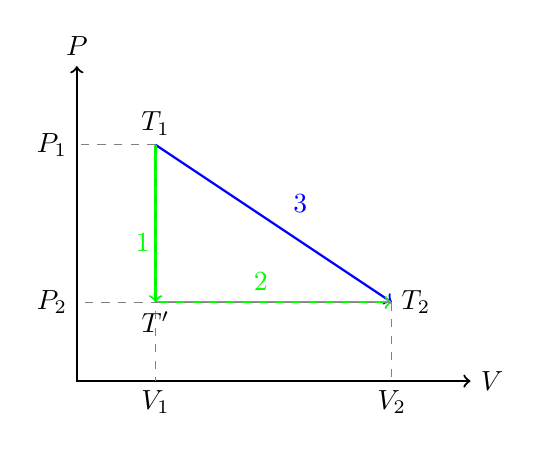
\begin{tikzpicture}[scale=1.0]
        % Draw axes
        \draw [<->,thick] (0,4) node (yaxis) [above] {$P$}
                |- (5,0) node (xaxis) [right] {$V$};
        \coordinate (f) at (4,1);
        \coordinate (m) at (1,1);
        \coordinate (i) at (1,3);
        \node [right] (lf) at (f) {$T_2$};
        \node [above] (li) at (i) {$T_1$};
        \node [below] (lm) at (m) {$T'$};
        \node [blue, label={[blue]10:$3$}] (label) at (2.5, 2) {};
        \draw [blue, thick, ->] plot [smooth, tension=1] coordinates { (i) (f)};
        \draw [green, thick, ->] plot [smooth, tension=1] coordinates { (i) (m)};
        \node [green, label={[green]10:$1$}] (label) at (0.5, 1.5) {};
        \draw [green, thick, ->] plot [smooth, tension=1] coordinates { (m) (f)};
        \node [green, label={[green]10:$2$}] (label) at (2, 1) {};
        \node [below] (vi) at (1,0) {$V_1$};
        \node [below] (vf) at (4,0) {$V_2$};
        \node [left] (pf) at (0,1) {$P_2$};
        \node [left] (pi) at (0,3) {$P_1$};
        \draw [gray, dashed] (i) -- (vi);
        \draw [gray, dashed] (i) -- (pi);
        \draw [gray, dashed] (f) -- (vf);
        \draw [gray, dashed] (f) -- (pf);
\end{tikzpicture}
\end{center}

Along the green path,

\[ \Delta S_1 = \intl \br{\f{\indif Q}{T}}_1 = C_v \intl_{T_1}^{T'} \f{\dif T}{T} = C_v \ln\br{\f{T'}{T_1}} \]
\[ \Delta S_2 = \intl \br{\f{\indif Q}{T}}_2 = C_p \intl_{T'}^{T_2} \f{\dif T}{T} = C_p \ln\br{\f{T_2}{T'}} \]

Thus the total change is given by,

\begin{align*}
\De S &= \De S_1 + \De S_2 \\
&= C_v \ln\br{\f{T'}{T_1}} + C_p \ln\br{\f{T_2}{T'}} \\
&= C_v \ln\br{\f{T'}{T_1}} + \br{C_v + R} \ln\br{\f{T_2}{T'}} \\
&= C_v \ln\br{\f{T_2}{T_1}} + R \ln\br{\f{T_2}{T'}} \\
&= \cancelto{0}{C_v \ln\br{\f{T_2}{T_1}}} + R \ln\br{\f{T_2}{T'}} \\
&= R \ln\br{\f{T_2}{T'}} \\
\end{align*}

Note the cancellation $T_1 = T_2$ since (3) is an isotherm. \\

Since path (2) is at constant $P$

\[ \De S = R \ln\br{\f{V_2}{V_1}} \]

Which is identical to the change in entropy along the isotherm derived above. Thus confirming that $\De S$ is independent of path.

\subsubsection{Clausius Inequality}

\begin{center}
\begin{tikzpicture}[
    scale=1.0,
    decoration={post length=1mm, pre length=1mm, markings, mark=at position 0.5 with {\arrow{>}}}
]
        % Draw axes
        \coordinate (nya) at (0, 0);
        \coordinate (pya) at (0, 4);
        \coordinate (nxa) at (0, 0);
        \coordinate (pxa) at (5, 0);
        \node [above] (lpya) at (pya) {$P$};
        \node [right] (lpxa) at (pxa) {$V$};
        \coordinate (a) at (1.2, 3);
        \coordinate (b) at (3.2, 2.2);
        \coordinate (c) at (4, 1);
        \coordinate (d) at (2, 1.5);
        \coordinate (ab) at (2.2, 2.4);
        \coordinate (bc) at (3.5, 1.5);
        \coordinate (cd) at (3, 1.15);
        \coordinate (da) at (1.5, 2.3);
        \draw [->, thick] (nya) -- (pya);
        \draw [->, thick] (nxa) -- (pxa);
        \draw [red, thick, postaction={decorate}] plot [smooth, tension=1] coordinates { (a) (ab) (b)};
        \draw [blue, thick, postaction={decorate}] plot [smooth, tension=1] coordinates { (c) (cd) (d)};
        \draw [thick, postaction={decorate}] plot [smooth, tension=1] coordinates { (b) (bc) (c)};
        \draw [thick, postaction={decorate}] plot [smooth, tension=1] coordinates { (d) (da) (a)};

        \node [above left] (la) at (a) {$a$};
        \node [above right] (lb) at (b) {$b$};
        \node [above right, red] (lab) at (ab) {$T_2$};
        \node [below left, blue] (lcd) at (cd) {$T_1$};
        \node [below] (lc) at (c) {$c$};
        \node [below left] (ld) at (d) {$d$};
\end{tikzpicture}
\end{center}

Recall from equation \eqref{eq:revcarnot}, we have that for a reversible Carnot cycle,

\[ \f{Q_2}{T_2} + \f{Q_1}{T_1} = 0  \]

Now consider the case of heat extraction and heat disposal along a \textit{tiny Carnot cycle}.

\[ \f{\indif Q_2}{T_2} + \f{\indif Q_1}{T_1} = 0  \]

\TODO{Insert PV circle liney diagram from notes he said he'd upload}

The idea here is to consider any physical process or cycle as being made up of numerous tiny adiabatic curves and isotherms. We \textit{approximate} the real cycle as being composed of a series of reversible processes. In the limit of the number of ``switches'' goes to infinity, the real engine process is made exactly reversible. \\

Essentially, we are mapping out the contour of any given cycle by following many isotherms and adiabats. Then for any given sub-process here,

\[ \sum_{i=1}^{n} \f{\indif Q_i}{T_i} = 0 \]

Or in the limit as $n \ar \inf$,

\[ \ointl \f{\indif Q\tsb{rev}}{T} = 0 \]

Again we observe that $Q\tsb{rev}/T$ is an \textbf{exact} differential and we can call it $\dif S$ as done before. $S$ is a state variable. \\

Any reversible cycle must obey the following equation,

\[ \ointl \f{\indif Q}{T} = 0 \note{For a reversible cycle.} \]

What about for an irreversible cycle? An irreversible cycle is some process that somewhat has a step that can not be performed backward. What we have shown is that the efficiency of an engine with an irreversible cycle $\eta'$ must be less than that of Carnot $\eta_C$ (see \eqref{eq:irreversiblecarnot}).

\[ \eta' < \eta_C\]

Using equation \eqref{eq:irreversiblecarnot}, we can show that,

\[ \f{Q'_1}{Q'_2} < \br{\f{Q_1}{Q_2}}\tsb{rev Carnot} \]

Or that,

\[ \f{\indif Q'_1}{T_1} + \f{\indif Q'_2}{T_2} < 0 \note{For an irreversible cycle.} \]

Which lead to the generalization for an infinite number of steps as,

\[ \sum_{i=1}^{n} \f{\indif Q'_i}{T_i} < 0 \ar \ointl \f{\indif Q'}{T} < 0  \]

This leads to the Clausius Inequality:

\[ \ointl \f{\indif Q'}{T} \leq 0 \]

Which achieves equality only when the \textbf{entire} cycle is irreversible. Inequality is always maintained if \text{any} part of the cycle is irreversible. This can be understood as another formulation of the Second Law of Thermodynamics. \\

There are two cases ``applications'' of Clausius inequality: \\

1) Consider a single two-step \textit{reversible} cycle

\begin{center}
\begin{tikzpicture}[
    decoration={post length=0.1mm, pre length=0.1mm, markings, mark=at position 0.5 with {\arrow{>}}}
]
\coordinate (1) at (0,0);
\coordinate (2) at (2,2);
\coordinate (A) at (0.8, 1.2);
\coordinate (B) at (1.2, 0.8);
\draw [blue, thick, postaction={decorate}] plot [smooth, tension=1] coordinates { (1) (A) (2)};
\draw [blue, thick, postaction={decorate}] plot [smooth, tension=1] coordinates { (2) (B) (1)};

\fill (1) circle (1pt) node[below left] {$1$};
\fill (2) circle (1pt) node[above right] {$2$};
\node [above left, blue] (lA) at (A) {$A$};
\node [below right, blue] (lB) at (B) {$B$};

\end{tikzpicture}
\end{center}

Therefore,

\[ \oint \f{\indif Q}{T} = 0 \]
\[ \intl_1^2 \br{\f{\indif Q}{T}}_A + \intl_2^1 \br{\f{\indif Q}{T}}_B = 0 \]

Rearrangement gives,

\[ \intl_1^2 \br{\f{\indif Q}{T}}_A = - \intl_2^1 \br{\f{\indif Q}{T}}_B = \intl_1^2 \br{\f{\indif Q}{T}}_B\]

Which implies that entropy is conserved,

\[ \br{S_2 - S_1}_A = \br{S_2 - S_1}_B \]

2) Consider a two-step \textit{irreversible/reversible} process

\begin{center}
\begin{tikzpicture}[
decoration={post length=0.1mm, pre length=0.1mm, markings, mark=at position 0.5 with {\arrow{>}}}
]
\coordinate (1) at (0,0);
\coordinate (2) at (2,2);
\coordinate (A) at (0.8,1.2);
\coordinate (B) at (1.2,0.8);
\draw [red, thick, postaction={decorate}] plot [smooth, tension=1] coordinates { (1) (A) (2)};
\draw [blue, thick, postaction={decorate}] plot [smooth, tension=1] coordinates { (2) (B) (1)};

\fill (1) circle (1pt) node[below left] {$1$};
\fill (2) circle (1pt) node[above right] {$2$};
\node [above left, red] (lA) at (A) {Irrev.};
\node [below right, blue] (lB) at (B) {Rev.};

\end{tikzpicture}
\end{center}

Therefore by the Clausius Inequality we have,
\[ \oint \f{\indif Q}{T} \leq 0 \]

\[ \ointl_1^2 \br{\f{\indif Q}{T}}\tsb{irrev} + \ointl_2^1 \br{\f{\indif Q}{T}}\tsb{rev} \leq 0 \]
\[ \ointl_1^2 \br{\f{\indif Q}{T}}\tsb{irrev} \leq - \ointl_2^1 \br{\f{\indif Q}{T}}\tsb{rev} = \ointl_1^2 \br{\f{\indif Q}{T}}\tsb{rev} \]

Thus we can conclude that with $\dif S \br{\f{\indif Q}{T}}\tsb{rev}$,

\[ \ointl_1^2 \br{\f{\indif Q}{T}}\tsb{irrev} \leq \ointl_1^2 \br{\dif S}\tsb{rev} = S_2 - S_1 \]

Which gives that our entropy increases each cycle,

\[ \br{S_2 - S_1}\tsb{rev} \geq \ointl_1^2 \br{\f{\indif Q}{T}}\tsb{irrev} \]

Now suppose that our system is undergoing an adiabatic process along the whole path. This means that no heat is exchanges during the process ($\indif Q = 0$). This gives us,

\[ \br{S_2 - S_1}\tsb{irrev} \geq 0 \note{For an irreversible, adiabatic process.}\]

In conclusion, the entropy can only increase for an \textit{isolated} (our adiabatic example) system undergoing an irreversible process. This is a restatement of the Second Law of Thermodynamics; entropy always increases for an isolated system. Of course this is all subject to the constraint imposed on the system: $N, V, E$ might be constrained or imposed to be constant. Or more clearly: \\

At \textit{equilibrium}, entropy must reach its maximum value. Otherwise it would increase because it has to.

\subsubsection{Perspective on Entropy}

Consider a container with two sub-sections. The left hand side will have a gas and the right hand side will have a vacuum (each side having volume $V$). At time $t=0$, the barrier between the two containers is removed and the gas has access to the entire container of volume $2V$. At equilibrium, the gas occupies the entire container. Evidently, this is an irreversible process (the gas does not have the luxury to return to it's original state). Some comments:

\begin{itemize}
    \item irreversible process
    \item gas does no work against the vacuum
    \item no heat exchange
    \item $\De U = \De Q - \De W = 0$ (Conservation of energy $\implies$ temperature is constant)
\end{itemize}

This process is irreversible, so there is no way to directly compute it's change in entropy throughout the entire process. However, the entropy can be calculated using properties about the two endpoints and a \textit{reversible} process that connects these endpoints. \\

The \textit{reversible} process we will consider as a replacement will be letting the gas expand via a piston held initially at the midway point of the container that is controlled externally. We will slowly move the piston until the gas fills the entire container. This new process is consider isothermal that takes use from state (1) (half gas, half vacuum) to state (2) (total gas). Along this process we can compute the change in entropy $S_2 - S_1$ along the reversible path. Turns out we already computed this in equation \eqref{eq:isothermvolumechangeentropy}.

\[ \De S = S_2 - S_1 = nR \ln\br{\f{V_2}{V_1}} \]

Let $nR = k_BN_A$ where $k_B$ is the Boltzmann constant and $N_A$ is Avogadro's number. Note that $V_1 = V$ and $V_2 = 2V$,

\[ \De S = k_BN_A \ln\br{\f{2V}{V}} = k_B \ln\br{2^{N_A}} \]

Thus we expect,

\[ \De S \propto \untext{\br{\text{const.}}}{units $J/K$} \times \ln \br{2^N} \]

Note that the `$2^N$' term measures the number of microstates that the system received or now has access to to due to the process. Consider the microstates counted by the possibility that the particle can be on the left or the right of the container.\\

\begin{itemize}
        \item All particles on left except 1
        \begin{itemize}
                \item LLLLL$\ldots$LLRLLL$\ldots$LLLLL
                \item $N$ ways for this to occur
        \end{itemize}
        \item All particles on the left except 2
        \begin{itemize}
                \item LLLLL$\ldots$LLRLLL$\ldots$LLRL$\ldots$LLLLL
                \item $N(N-1)/2$ ways for this to occur
        \end{itemize}
\end{itemize}

The most probable macrostate occurs when the total number of microstates reaches a maximum. Using the Stirling's approximation, this occurs when there is a 50/50 split between the left and right with total number of microstates,

\[ \Om \sim 2^N + \text{small corrections} \]

Note that disordered (``mixed'') states (50/50) can be realized in so many more ways than ``ordered states''. \\

With this view, entropy can be viewed as a measure of the number of microstates through the rational of the second law. These ideas are what lead Boltzmann to consider the possibility,

\[ S \sim \ln \Om \]

With further corrects and units,

\[ S = k_B \ln \Om +S_0 \]

Where the constant $S_0$ can be shown to be zero with the Third Law of Thermodynamics.

\subsubsection{Conclusion}

The Second Law of Thermodynamics is very much a manifestation of the probability/statistics of the large number of states microscopic objects can realize. \\

The law $\De S \geq 0$ spontaneously for an isolated system means that we must seek microscopic configurations that \textit{maximize} S, as when this is achieved, the system must have reached equilibrium.

\section{S.M. Basis for T.D.}

Statical Mechanics Basis for Thermodynamics.

\subsection{Contact Between S.M. \& T.D.}

\begin{enumerate}
        \item Systems where $V \ar \inf$ and $N \ar \inf$ and the density $N/V$ remains constant
        \begin{itemize}
                \item Thermodynamically large system
        \end{itemize}
        \item Equilibrium Thermodynamics / S.M.
        \begin{itemize}
                \item Consider two regions $(1,2)$ of a container separated by a diathermal wall
                \item $(N_1, V_1, E_1)$ and $(N_2, V_2, E_2)$ number of particles, volume, energy respectively
                \item Interested in total number of microstates
                \item Composite system $\Om^{(0)} = \Om^{(1)} \times \Om^{(2)}$
        \end{itemize}
\end{enumerate}
This composite system has $E^{\br{0}} = E_1 + E_2 = $ constant. We are interested in $\Om$: the number of microstates. At \textit{any time}, system (1) is just as likely to be in any of its microstates. This is also true for system (2).
\[ \Om^{(0)}\br{E_1, E_2} = \Om_1(E_1) \times \Om_2(E_2) \]
\[ \Om^{(0)}\br{E_1, E^{(0)} - E_1} = \Om_1(E_1) \times \Om_2(E^{(0)} - E_1) \]
The most likely macrostate is the one with the most number of microstates. It is important to note that is true at \textit{any time}. To maximize $\Om^{(0)}$,
\[ \pder{\Om^{(0)}}{E_1} = 0 \implies \bre{\pder{\Om_1}{E_1}}_{E_1 = \bar{E}_1} \Om_2(\bar{E}_2) + \Om_1(\bar{E}_1) \bre{\pder{\Om_2}{E_2}}_{E_2 = \bar{E}_2} \pder{E_2}{E_1} = 0 \]
Note since $E^{(0)}$ is fixed,
\[ \pder{E_2}{E_1} = -1 \]
Which reveals,
\[ \f{1}{\Om_1(E_1)} \bre{\pder{\Om_1}{E_1}}_{E_1 = \bar{E}_1} = \f{1}{\Om_2(E_2)} \bre{\pder{\Om_2}{E_2}}_{E_2 = \bar{E}_2} \]
Notice the logarithmic nature of this equation to show that,
\[ \underbrace{\bre{\pder{\ln\Om_1}{E_1}}_{E_1 = \bar{E}_1}}_{\be_1} = \underbrace{\bre{\pder{\ln\Om_2}{E_2}}_{E_2 = \bar{E}_2}}_{\be_2} \]
Therefore in summary, equilibrium requires $\be_1 = \be_2$. Recall that for a reversible process,
\[ \dif U = \indif Q - \indif W \]
Thus,
\[ \dif E = \indif Q - \indif W \]
\[ \dif E = T \dif S - P \dif V \]
Where the definition of entropy can be expressed,
\[ \pdert{S}{N,V}{E} = T \]
Which gives for system 1,
\[ \br{\pder{E_1}{\ln\Om_1}} \br{\pder{\ln\Om_1}{S_1}} = T_1 \]
And the analogous expression for system 2,
\[ \br{\pder{E_2}{\ln\Om_2}} \br{\pder{\ln\Om_2}{S_2}} = T_2 \]
Combining these two systems gives,
\[ \pder{S_1}{\ln\Om_1} = \f{1}{\be_1T_1} \qquad \pder{S_2}{\ln\Om_2} = \f{1}{\be_2T_2} \numberthis \label{eq:entropymotiv}\]
Equations \eqref{eq:entropymotiv} should be telling for the following assumption. \\

\textbf{Assumption:} There exists an intimate relationship between Statistical Mechanics and Thermodynamics for all and any system. \\
We will propose that,
\[ \f{1}{\be_1T_1} = \f{1}{\be_2T_2} = \f{1}{\be T} = \text{ constant/universal } \]
Thus,
\[ S = \text{constant}\cdot \ln \Om \numberthis \label{eq:blankboltzmann} \]
Where the unknown constant is actually Boltzmann's constant, $k_B$ with,
\[  \be = \f{1}{k_B T} \]
What about the relationships between other quantities associated with systems (1) and (2)? First consider volume.

\[ \underbrace{\bre{\pder{\ln \Om_1}{V_1}}_{N_1, E_1, V_1 = \bar{V}_1}}_{\eta_1} = \underbrace{\bre{\pder{\ln \Om_2}{V_2}}_{N_2, E_2, V_2 = \bar{V}_2}}_{\eta_2} \]
Which gives,
\[ \eta_1 = \eta_2 \]

These new variables describe the equilibrium of the two systems in terms of volume. Is it required to introduce a new constant similar to above to relate volume to entropy? Consider,
\[ \dif E = T \dif S - P \dif V \numberthis \label{eq:nonchempot}\]
Thus,
\[ \pder{S}{E} = \f{1}{T} \qquad \pdert{S}{V}{E} = \f{P}{T} \]

However, we could introduce another term to \eqref{eq:nonchempot} to include flux of particles; a chemical potential term. We could add more terms,

\[ \dif E = T \dif S - P \dif V  + \mu \dif N - H \dif M\]
Which would produce more relations like,
\[ \pder{S}{N} = - \f{\mu}{T}\]

From this we get,

\[ \pder{\ln\Om}{V} = \eta \]

Which by chain rule,

\[ \pder{\ln\Om}{S}\pder{S}{V} = \eta \]

But we know from \eqref{eq:entropymotiv} that $\pder{\ln\Om}{S} = \be T$. Therefore,

\[ \pder{S}{V} = \f{1}{\be T} \eta = \f{P}{T} \]

Therefore rearrangement gives,

\[ \eta = \f{P}{k_B T} \]

In summary, once we have the result \eqref{eq:blankboltzmann}, with the universal constant $k_B$, all expected equilibrium between generalized forces must be satisfied. No new constants or relations need to be constructed to explore the relationship between entropy and microscopic quantities. \\

An equilibrium of energy and volume between systems (1) and (2) it must be that,
\[ T_1 = T_2 \qquad P_1 = P_2 \]

Furthermore, and equilibrium of energy and number of particles it must be that,
\[ T_1 = T_2 \qquad \mu_1 = \mu_2 \]

\textbf{Remark:} Equilibrium properties in the extensive ($E, V, N$) variables of the system translate in an equally in the intensive $(T, P, \mu)$ variables. \\

In summary, the equation $S = k_B \ln \Om$ recovers all expected descriptions of thermodynamical equilibrium.

\subsection{Classical Ideal Gas from S.M.}

For this analysis, we will begin with the consideration at $\hbar = 0$. In other words, we will consider the particles to point like and ignore their wave like nature and treat interactions between particles ($V(r_{ij})$) is very small. Note however, in physics, one cannot claim something is ``small'' unless the quantity is dimensionless. Everything is small compared to something else. Thus when we say $\hbar$ is small, we mean that the DeBrogile wavelength is small compared to the thermal length scale. Similarly for the potential energies between the particles, $V/k_BT \ll 1$. \\

\subsubsection{Volume}
Consider the volume the gas occupies as a fixed volume $V$. Also notice that it is acceptable at this point to say that the number of microstates is proportional to the volume.

\[\Om \propto V^N \]

Where $N$ is the number of particles. But how can be compare microstates which are dimensionless to the volume which could have dimensions $m^3$? In practice we assume,

\[ \Om = \text{ constant } \times \br{\f{V}{\Lambda^3}}^N \]

Where $\Lambda$ is a length scale of the system. We will return to this idea later when considering quantum gases. Note from above, we have,

\[ \pdert{S}{V}{E} = \f{P}{T} \]

Combined with $S = k_B\ln\Om$ and $\Om = c V^N$,

\[ PV = N k_B T \]

This is quite remarkable. We just derived an expression for an ideal gas using $S = k_B\ln\Om$ and some simple motivations for the form of $\Om$. Typically, this ideal gas law is written with,

\[ N k_B = N_A R \]

Where $N_A$ is Avogadro's number $\SI{6.02e23}{}$ and $R$ was known that $R = \SI{8.31}{\J\per\mole\per\K}$ which gives a value for,

\[ k_B = \SI{1.38e-23}{\J\per\K} \]

\subsubsection{Energy \& Particle in a Box}

As a reminder, an ideal gas has no interaction $V=0$ and modeling the particles as particles in a box. As such, they are fundamentally quantum mechanical in nature. For a particle in a box, recall from Q.M. that for a potential,

\[ U(x) = \piecewise{0}{0 \leq x \leq L}{\inf}{\text{otherwise}} \]

The energy is given by,
\[ H = \f{p^2}{2m} \]

Where,

\[ \vec{p} = \f{\hbar}{i} \vdel \qquad H = -\f{\hbar^2}{2m}\del^2\]

The Time Independent Schrödinger Equation (TISE) gives,

\[ H \psi = \vep \psi \]

We can use this to find the energy $\vep$,

\[ -\f{\hbar^2}{2m}\del^2 \psi = \vep \psi \]

Which yields generic solution,

\[ \psi = A \sin \br{kx} \]

Where $k L = n \pi$ and $A = \sqrt{2/L}$ and the energy in the $n$-th state is given by,

\[ \vep = \f{\hbar^2}{2mL^2} \pi^2 n^2 \note{For 1D box}\]

However, the generalization for 3d space $\R^3$, the energy is determined by three quantum numbers $(n_x, n_y, n_z)$ all strictly positive integers $\Z_{>0}$,

\[ \vep = \f{\hbar^2}{2mL^2} \pi^2 \bc{n_x^2 + n_y^2 + n_z^2}\]

This energy $\vep$ is characterized by $3$ independent integers -for a single particle. For $N$ particles in this box $V = L^3 \subset \R^3$ we will require $3N$ independent numbers. Classically, the Lagrangian of the system is,

\[ L = T - V \]

Where $T$ is the kinetic energy and $V$ is the potential energy. The kinetic energy is given by,

\[ T = \f{p_x^2}{2m} + \f{p_y^2}{2m} + \f{p_z^2}{2m} \]

Evidently for a single particle, $n$ cannot be zero because then that would yield the trivial solution $\psi(x) = 0$. So why is it that for the 3d example, it is still required that $n_x, n_y, n_z > 0$ and each cannot equal zero? It is because the solution is solved using separation of variables. In any of the components of the solution are the trivial solution $n_i = 0$ for a particular $i$, the complete solution becomes the trivial solution. \\

Therefore using this three number $n_x, n_y, n_z$, we can describe the energy of a given particle for all time. However, for a fixed $\vep$ that can be measured, how many distinct set of $n_i$'s can produce this measured energy $\vep$?

\[ \f{\hbar^2}{2mL^2} \pi^2 \bc{n_x^2 + n_y^2 + n_z^2} = \vep\]

Since the $n_i$'s are integers, solving this problem for a fixed $\vep$ is the same as solving the Diophantine equation,

\[ x^2 + y^2 + z^2 = R^2 \numberthis \label{eq:spheredio}\]

Which geometrically is equivalent to asking the question:\\

\textit{Where does the surface of the sphere intersect with a 3d grid of unit spacing?} \\

Therefore, the total number of microstates for a fixed energy $\vep$ is the same as determining the number of solutions to \eqref{eq:spheredio}. Let us call,

\[ \vep^* = \f{2m}{\hbar^2\pi^2}V^{2/3} \vep \]

Where $\vep^*$ acts as a dimensionless energy that characterizes the problem ($R^2 = \vep^*$).

\[ \Om = \text{\# of solutions to \eqref{eq:spheredio}} \]

In general (like all Diophantine equations), this problem is very hard. It is known as the \textbf{microcanonical ensemble} problem.

\subsection{Microcanonical Ensemble}

The Microcanonical ensemble problem involves finding positive integers $n_x, n_y, n_z$ such that,
\[ n_x^2 + n_y^2 + n_z^2 = \f{2mL^2}{\hbar^2 \pi^2} \vep = \f{2mV^{2/3}}{\hbar^2 \pi^2} \vep \defined \vep^* \]
Classically the total energy energy of the system is given by the sum of the kinetic energies of each of the particles.
\[ E = K_1 + K_2 + K_3 + \cdots + K_N \]
Which when broken into each component,
\[ E = \br{\f{p_{1x}^2 + p_{1y}^2 + p_{1z}^2}{2m}} + \br{\f{p_{2x}^2 + p_{2y}^2 + p_{2z}^2}{2m}} + \cdots + \br{\f{p_{Nx}^2 + p_{Ny}^2 + p_{Nz}^2}{2m}} \]

For fixed $E$ in general, this constitutes a $3N$ dimensional problem,
\[ \sum_{i=1}^N \f{\hbar^2 \pi^2}{2 m V^{2/3}} \br{n_{ix}^2 + n_{iy}^2 + n_{iz}^2} = E \]

Which can be expressed with shorthand notation as,
\[ \sum_{r=1}^{3N} \f{\hbar^2 \pi^2}{2 m V^{2/3}} n_{R}^2 = E \]

Where $n_{R}$ is the $r$-th degree of freedom of the system. This can be express even more compactly by absorbing constants,
\[ \sum_{r=1}^{3N} n_{R}^2 = E^* \defined E \f{2 m V^{2/3}}{\hbar^2 \pi^2} \numberthis \label{eq:canonensemble} \]

Notice that the term $E V^{2/3}$ completely characterizes the number of microstates $\Om$ as it determines the number of solutions of \eqref{eq:canonensemble}. What we notice that without calculating $\Om$, we can determine the form of entropy.

\[ S = S\br{N,V,E} = S\br{N, E V^{2/3}} \]

For a system undergoing a reversible adiabatic change, we have both $\indif Q = 0$ which implies that $\dif S = 0$ for fixed temperature which implies that entropy is constant. Therefore for a reversible adiabatic process, in order to ensure that entropy is constant, it must be that,
\[ V^{2/3} \cdot E = \text{const.} \note{For reversible/adiabatic process} \]

Now using the known expression,

\[ P = - \pdert{E}{V}{N,S} \]

And using $c$ as a constant,

\[ E = c V^{-2/3} \]

Which gives,
\[ PV^{5/3} = \text{constant} \note{For reversible/adiabatic process.} \]

Or more generally, for quantum/classical systems,

\[ PV^\ga = \text{constant} \note{$\ga = 5/3$ for monoatomic system} \numberthis \label{eq:adiabtic} \]

Note that \eqref{eq:adiabtic} does not hold for relativistic systems as $E = pc$ where $c$ is the speed of light.

\subsubsection{Solving the Microcanonical Ensemble}
\label{sec:solvemircoensemble}

One will notice that as $E^*$ increases, the number of solution $\Om$ varies wildly. It can be precisely $0$ and some values for $E^*$ and very many for other, nearby energies. Instead of calculating only the $n_r$ for which $E$ is precisely given, we will instead compute all the states for which $E' < E$ to simplify the problem. In principle, we want to replace the problem of finding,

\[ \Om(N, V, E) \]

We will instead compute (for 1 particle),

\[ \sum_{'} \br{\vep'} = \sum_{\vep' \leq \vep} \Om(1, V, \vep') \]

Where,

\[ \sum_{n_r'}^{3} n_r^2 = \vep^* \]

Which can be converted to a continuous problem of calculating the volume of this sphere,
\[ \intl_V \dif V \]

Which is a problem of finding the volume of a sphere of radius $\sqrt{\vep^*}$. In this case of 1 particle, $V$ has dimension $3$. Therefore,

\[ V(R) = \f{4 \pi R^3}{3} \]
\[ V(\vep^*) = \f{4 \pi }{3}\br{\vep^*}^{3/2} \]

Now since we only care about the cases where $n_x, n_y, n_z$ are positive, this quantity \textit{overestimates} by $2^3= 8$ times the desired amount. Therefore the sum over all states where $0 \leq \vep'\leq\vep^*$ is

\[ \sum_{'} = \f{1}{8} \f{4\pi}{3} \br{e^*}^{3/2} = \f{\pi}{6} \br{e^*}^{3/2} \]

Now we must repeat this calculation for not a 3d sphere but a 3Nd-sphere.

\heading{Mathematical Interlude}

In 3-d, a volume element is given by, $\dif V = \dif x \dif y \dif z \defined \dif x_1\dif x_2\dif x_3$. \\

In n-d, a volume element is given by,

\[ \dif V_n = \prod_{i=1}^{n} \dif x_i \]

Therefore in n-d the volume of a sphere is given by,

\[ V_A = \intl \dif^n r = \intl \cdots \intl \dif x_1 \dif x_2 \cdots \dif x_n = \intl \cdots \intl \prod_{i=1}^{n} \dif x_i \]

And performing this sum under the constraint that,

\[ 0 \leq \sum_{i=1}^{n} x_i^2 \leq R^2 \]

\begin{center}
\begin{tabular}{|c|c|}
        \hline
        Dimensions & Volume of Ball \\
        \hline
        $2$ & $\pi R^2$ \\
        $3$ & $\f43 \pi R^3$ \\
        $\cdots$ & $\cdots$ \\
        $n$ & $c_n R^n$ \\
        \hline
\end{tabular}
\end{center}

Therefore, we need to find $c_n$ in general to get the volume of a hypersphere. Since $V_n = c_n R^n$, consider

\[ \dif V_n = \dif \br{c_n R^n} = \underbrace{c_n \cdot n \cdot R^{n-1}}_{S_n} \dif R \]

\textbf{Trick:} We will take a function that we like for which we can do exactly the integrals in $\dif x_i$ (i.e. Cartesian Coordinates) and perform the integral in spherical coordinates.

\[ \intl f(\bc{x_i}) \prod_{i=1}^n \dif x_i = \intl f(R) S_n \dif R = \intl f(R) n c_n R^{n-1} \dif R \]

Now make use of Gaussian integrals used in section \ref{sec:gaussianintegrals},

\[ f(x) = e^{-x^2} \]
\[ f(\bc{x_i}) = \prod_{i=1}^{n} e^{-x_i^2} \]

Gives,

\[ \intlf e^{-x^2} \dif x = \sqrt{\pi} \]

Which for generic $n$ with separating the terms $x_i$ gives,

\[ \prod_{i=1}^{n} \intlf e^{-x_i^2} \dif x_i = \intlf e^{-x_1^2} \dif x_1 \intlf e^{-x_2^2} \dif x_2 \cdots \intlf e^{-x_n^2} \dif x_n = \intl_0^{\inf} f(R) n c_n R^{n-1} \dif R \]

The RHS has $n$ terms that each evaluate to $\sqrt{\pi}$,

\[ \pi^{\f{n}{2}} = \intl_0^{\inf} f(R) n c_n R^{n-1} \dif R = n c_n \intl_0^{\inf} f(R) R^{n-1} \dif R \]

Since $f(R)$ is just a Gaussian in $R$,

\[ \pi^{\f{n}{2}} = n c_n \intl_0^{\inf} e^{-\br{\sum_{i=1}^{n}x_i^2}} R^{n-1} \dif R = n c_n \intl_0^{\inf} e^{-R^2} R^{n-1} \dif R \]

Using the identity,

\[ \intl_0^{\inf} e^{-\al y^2} y^\nu \dif y \defined \f{1}{2\al^{\f{\nu+1}{2}}}  \Ga\br{\f{\nu +1}{2}} \note{For $\nu > -1$}\]

Where $\Ga(x)$ is the \textit{Gamma function} which is equivalent to factorials for $x$ integers, we get,

\[ \pi^{\f{n}{2}} = n c_n \f12 \Ga \br{\f{n}{2}} \]

Thus,

\[ c_n = \f{\pi^{\f{n}{2}}}{\br{\f{n}{2}}!} \]

Therefore,

\[ V_n (R) = \f{\pi^{\f{n}{2}}}{\br{\f{n}{2}}!} R^n \]

Therefore for $n = 3N$ and $R = \sqrt{E^*}$ the total number of states contained inside the hypersphere with radius $R$ is given by,

\[ {\sum}_N (N, V, E) = \br{\f{V}{h^3}}^N \f{\br{2\pi m E}^{3N/2}}{\br{\f{3N}{2}}!} \]

Where ${\sum}_N$ doesn't explicitly represent a \textit{sum}. Instead it is the total number of microstates within the hypersphere. It is a \textit{function} of $N, V, E$. Note this includes the factor of $\f12^{3N}$ to only count the positive integer solutions.\\

What we want to do is to derive the thermodynamic properties for E. In reality however, no system is perfectly isolated from surroundings. In practice $E$ is not exactly defined. We will construct the idea of $\De$ or uncertainty in $E$ is only because of the imperfect nature of the system. Assume that the energy is given by $E \pm \f{\De}{2}$. We will also assume that $\De \ll E$. Since initially we wanted to know $\Om(N, V, E)$ we really want to know the the number of states associated with a measure of the energy within the uncertainty. This will be the difference of two ${\sum}_N$ values.

\[ \Ga_{N, V, \bar{E} = E} = {\sum}_N \br{N, V, E + \f{\De}{2}} - {\sum}_N \br{N, V, E - \f{\De}{2}} \numberthis \label{eq:deltaE}\]

Now in the limit that $\De/E \ar 0$,

\[ \lim_{\De/E \ar 0} \Ga_{N, V, \bar{E} = E} = \Ga_{N, V \bar{E} = E} = \lim_{\De/E \ar 0} \bs{{\sum}_N \br{N, V, E + \f{\De}{2}} - {\sum}_N \br{N, V, E - \f{\De}{2}}} = \pder{{\sum}_N}{E} \cdot \De \]

Therefore the total number of states associated with $E= \bar{E}$ is given by,

\[ \Ga_{N, V, \bar{E} = E} = \pder{\sum_N}{E} \cdot \De = \f{3N}{2} \f{\De}{E} \sum_N(N, V, E =\bar{E}) \]

Using the Boltzmann equation for entropy and Stirling's approximation with $N \gg 1$ (see section \ref{sec:stirling}),

\[ S = k_B \ln\Ga_N = k_B \bs{N \ln \bc{\f{V}{h^3} \br{\f{4\pi m E}{3N}}^{3/2}} + \f{3N}{2} + \bc{\ln \br{\f{3N}{2}} + \ln \br{\f{\De}{E}}}}  \]

This gives us the entropy of an ideal gas at energy $E$ within a window $E \pm \De /2$.\\

What thermodynamic properties does this expose?
\[ S(N,V,E) = k_B \ln\Ga_N \approx k_B \bs{N \ln \bc{\f{V}{h^3} \br{\f{4\pi m E}{3N}}^{3/2}} + \f{3N}{2}} \numberthis \label{eq:notextensive} \]

Notice that this depends on $\ln(N)$ and also $N^{-3/2}$ which seems to indicate that theses are not extensive variables. We will return to this problem soon. Rearranging for energy,

\[ E(S, V, N) = \f{2h^2N}{4 \pi m V^{2/3}} \exp\br{\f{2S}{3Nk_B} - 1} \]

Thermodynamically, we have,
\[ T = \pdert{E}{S}{V,N} \]

Which reveals,
\[ E = N \br{\f32 k_B T} \]

And the heat capacity at constant volume is given by,
\[ c_V = \pdert{E}{T}{N,V} = \f32 N k_B = \f32 nR \]

And analogously,
\[ c_P = T \pdert{S}{T}{N,P} = \f53 N k_B \]

Furthermore, thermodynamic pressure is given by,
\[ P = -\pdert{E}{V}{N,S} = \f23 \f{E}{V} \]

Combining these two results, we can see that,
\[ PV = nRT \]

Which means we have recovered all known results for ideal gases from only the \textit{explicit} form of $\sum_N$ (or $\Ga_N$).\\

Consider an isothermal change of entropy of entropy, and we recover,

\[ S_2 - S_1 = N k_B \ln\br{\f{V_2}{V_1}} \]

Or for a reversible adiabatic change/process,
\[ E,T \sim V^{-2/3} \]
\[ PV^\ga = \text{const.} \]
\[ TV^{\ga -1} = \text{const.} \]

We also recover that,

\[ \dif E = -p \dif V = -\f23 \f{E}{V} \dif V \]

In conclusion we have discovered that measuring and counting microstates $\Om_N \approx \sum_N, \Ga_N$ we can then use $S = k_B \ln \Om$ to recover and describe thermodynamic properties. All that remains is to discuss the problem that $V$ and $N$ do \textit{not} appear to be extensive variables in equation \eqref{eq:notextensive}. This problem is known as \textbf{Gibb's Paradox}.

\subsection{Gibb's Paradox}
How can we fix or understand the origin of the lack of extensivity in the formula $S = k_B \ln \Om$? We should expect $S$ to scale with $V$ but in \eqref{eq:notextensive} it does not. Does this mean that \eqref{eq:notextensive} is somehow wrong? \\

To expose this paradox, consider a container segmented by a wall into 2 regions with properties $N_1, V_1, T_1$ and $N_2, V_2, T_2$ with total volume $V = V_1 + V_2$. Now measure the entropy using \eqref{eq:notextensive} for each system $S_1$, $S_2$ and then adiabatically remove the wall between the segments of the container and recalculate entropy $S_T$ of the combined system. Does $S_T = S_1 + S_2$?

Using $E = \f32 N k_B T$

\[ S_i = N_i k_B \ln V_i + \f32 N_i k_B \bc{1 + \ln\br{\f{2 \pi m_i k_B T}{h^2}}} \quad i = 1,2 \]

While,

\[ S_T = \sum_{i=1}^{2} N_i k_B \ln V\]

Consider the case where the particle densities are the same and thus is also the same for the mixture after removing the wall.

\[ \f{N_1}{V_1} = \f{N_2}{V_2} = \f{N_1+ N_2}{V_1 + V_2} \]

Therefore the change in entropy is given by,

\[ \De S = S_T - \br{S_1 + S_2} \]

Which is explicitly,

\[ \De S = k_B \bc{N_1 \ln\br{\f{N_1 + N_1}{N_1}} + N_2\ln\br{\f{N_1 + N_1}{N_2}}} \numberthis \label{eq:entropyup} \]

Now lets assume $m_1 = m_2$ or that we have identical particles. From this, the macrostate of the system looks like it doesn't change when the wall is removed by we still have by equation \eqref{eq:entropyup} that,

\[ \De S > 0 \]

This makes no sense because if the particles are the same, we have not \textit{mixed} anything. \\

The resolution is to write (using Stirling's formula),

\[ \De S = k_B \bc{\ln \bs{\br{N_1 + N_2}!} - \ln \bs{N_1!} - \ln \bs{N_2!}} \]

To fix this problem we need to reduce $S$ or $\Om$ by a factor of $N!$.

\[ S \text{ reduced by } k_B \ln N!\]
\[ S_1 \text{ reduced by } k_B \ln N_1!\]
\[ S_2 \text{ reduced by } k_B \ln N_2!\]

This is an \textit{ad hoc} fix. It does not have any profound explanation of justification. The mechanism that describes this, is the notion of indistinguishably. The notion of indistinguishably is needed to be taken into account in order to properly count the number of microstates of a system. Proper analysis of this idea requires the theory of Quantum Statistics. Now we can go back and determine the proper formula for \eqref{eq:notextensive}.

\[ S(N,V,E) = N k_B \ln\br{\f{V}{N}} + \f{3Nk_B}{2} \bc{\f53 + \ln\br{\f{2 \pi m k_B T}{h^2}}} \]

This is the formula for the entropy of a non-degenerate ideal gas. This is known as the \textbf{Sackur-Tetrode equation}. One should note that this equation is quite remarkable. It is composed of only $N, V, E$ and a set of constants. This equation gives a proper extensivity of $S$. \\

For more, look at the theory of super-solid helium.

\section{Ensemble Theory}

Let's step back and review some of the statements we have made. Here are come general facts:
\begin{itemize}
    \item Every microstate has equal probability of being selected
    \item As time passes, the system will explore all of the microstates
    \item Experimental measurements are made of the time averaged of the true, non-stationary value of physical quantities $f$
    \begin{itemize}
        \item $f = E, \text{pH}, \text{etc.}$
        \item For example, measuring the pH level of a chemical solution will be the average measure over a macroscopic duration of time
        \item For systems where the dynamics of the system have time scale much shorter than the measurement frequency, the measured quantity ends of being an averaged value
    \end{itemize}
    \item Making a ``movie'' of a physical system (many measurements) and replacing the time average by a ``still frame'' average
    \begin{itemize}
        \item $\bs{f}\tsb{time} = \f1T \intl_{t_0}^{t_0 + T} f(t) \dif t$: the square brackets with subscript time indicate an average measure over time
        \item $\ba{f}\tsb{exp} = \bs{f}\tsb{time}$: Natural one should expect the time averaged value to be measure experimentally
        \item In doing thus, there must be some sort of averaging of the true real-time value using ``snapshots'' of $f$
    \end{itemize}
\end{itemize}
The question becomes, what are the options for performing this ``snapshot'' averaging? One could make periodic snapshots at fixed frequency or random intervals or combinations there of. It is the spirit of ensemble theory to determine how to construct an adequate way to compute $\ba{f}\tsb{exp}$ withing explicitly doing $\int f(t) \dif t$. Some options include,
\begin{itemize}
    \item microcanonical ensemble
    \item canonical ensemble
    \item grand ensemble
\end{itemize}
The procedure introduced by Gibb's involves utilizing phase space and classical systems.\\

\textbf{Remark by \AuthorName:} This is intimately connected to the \textit{Erdős discrepancy problem}. (I think?)

\subsection{Phase Space of Classical System}
\subsubsection{Dynamics \& Phase Space}

Imagine we have a system of $N$ \textit{distinguishable} particles,
\[ i = 1,2,3,\ldots,N \]
that lives in the space of 3 dimensions $\R^3$. We will fix for the system $N,V,E$. This is a microcanonical system/construction. We will also consider for the system that the particles are localized (they are were they are) and they do move (they have dynamics). The position of a particle $\mu$ is given by,
\[ \vr_\mu = x \hx + y \hy + x \hz \]
And each particle $\mu$ has same mass $m$. The momentum of particle $\mu$ is given by,
\[ \vp_\mu = m \dvec{r}_\mu \]
To index the entire system of $N$ particles, we will consider this index map,
\[ \vr_\mu = r_{\al,\mu} \mapsto r_i \quad \al = 1,2,3 \quad  \mu = 1,2,\ldots, N \quad  i = 1,2,\ldots,3N \]
Similarly for $\vp_\mu$
\[ \vp_\mu = p_{\al,\mu} \mapsto p_i \quad \al = 1,2,3 \quad  \mu = 1,2,\ldots, N \quad  i = 1,2,\ldots,3N \]
The product of the two spaces $\bc{r_i} \times \bc{p_i}$ is a $6N$ dimensional space known as the \textbf{phase space} of the system. To determine the dynamics of the system, we need to solve the following problem.
\[ \mathcal{L} = K\br{\bc{\dot{q}_i}} - V\br{\bc{q_i, \dot{q}_i}} \]
Where $\mathcal{L}$ is the \textbf{Lagrangian}, $K$ is the kinetic energy that depends on velocities, and $V$ is the potential energy which depends on position and sometimes velocities. Will will make the switch to the \textit{Hamiltonian} formalism of classical mechanics through a \textbf{Legendre Transform},
\[ H = \sum_{i}^{3N} \dot{q}_i \pder{\mathcal{L}}{\dot{q}_i} - \mathcal{L} = \sum_{i}^{3N} \dot{q}_i p_i - \mathcal{L} \]
Where $p_i = \pder{\mathcal{L}}{\dot{q}_i}$ is the generalized momentum. In principle, all classical problems can be described under this formalism. The ``bottle neck'' of this formalism is typically solving the equations of motion,
\[ \dot{p}_i = - \pder{H}{q_i} \qquad \dot{q}_i = \pder{H}{p_i} \numberthis \label{eq:hamiltonmechanics} \]
For generic physical quantity $f\br{q,p;t}$ that depends on time, positions an momentum of all the particles, all that would be required is to solve the equations of motion, and predictions could be made. However, this is very \textit{difficult}. Ensemble Theory allows for the construction of proper approximations for generic $f$. \\

\heading{$\mu$-space vs. $\Ga$-space}

We will now introduce the notion of $\mu$-space. In this $6N$ dimensional space, we assign to each particle $\mu$ a single point,

\[ \vr_\mu , \vp_\mu \mapsto \br{r_x, r_y, r_z, p_x, p_y, p_z} \]

For $N$ particles, there are $N$ points in the $\mu$-space which are characterized by $6N$ numbers. The alternative description is phase space ($\Ga$-space). Points in phase space are representative points on the \textit{entire} system at once,
\[ \text{state vector} = \br{q_1, q_2, \ldots , q_{3N} ; p_1, p_2, \ldots , p_{3N}} \]
At a given time $t$, there is $1$ point in phase space that is $6N$ dimensional. We will subscribe to the notation,
\[ \br{q_i\br{t}, p_i\br{t}} = \br{q,p} \]

\subsubsection{Trajectories in Phase Space}
How can be discuss or describe the time evolution of the system using phase space? The state vector of the system $\br{q,p}$ changes over time and this describes how each and every particles position and momentum changes with time.\\

As a function of time, the representative point traces a trajectory which \textbf{never} intersects itself. This is because the time evolution of the system is governed by the Hamiltonian $H$ and the solutions to the equations of motion are unique for given initial conditions. If there were intersection, take the intersection point as the initial condition and there would be two potential trajectories available for the system. Note however, that the system can loop back on itself and form cyclic trajectories. \\

Furthermore because of the fixed energy $E$ condition, there is a loss of 1 degree of freedom. Thus the trajectory is constrained to a $\br{6N-1}$ dimensional surface or hypersurface. Similar to the microcanonical ensemble problem solved in section \ref{sec:solvemircoensemble} (specifically equation \eqref{eq:deltaE}), we will treat this hypersurface or hypershell as a volume between the surfaces prescribed by the two energies,
\[ E + \f{\De}{2}, E - \f{\De}{2} \]

In general, the representative points $\br{q,p}$ are bounded. The positions $q$ are bounded by volume and the momentums $p$ by total energy through $K = \f{p^2}{2m}$.\\

\textbf{Remark:} One refers to classical solutions for ``real particles'', as opposed to \textit{virtual particles} (\textit{off shell}), as being \textit{on shell}, meaning they are found \textit{exactly} on the hypersurface defined by fixed energy $E$. \\

\subsection{Essential Replacement for Ensemble Theory}

So what do we mean when discussing ``ensembles''? Well one thing to notice is there a issue of difficulty with trying to solve the equations of motion \textit{explicitly}. We would like to instead compute a notion of average,
\[\ba{f(q,p)}\tsb{exp} = \f{1}{T} \intl_{t_0}^{t_0 + T} f\br{q(t),p(t)} \dif t \]
Where $T$ is a duration that is ``long enough''. The equations of motion for the system are given by Hamiltonian mechanics \eqref{eq:hamiltonmechanics},
\[ \dot{q}_i = \pder{H}{p_i} \qquad \dot{p}_i = -\pder{H}{q_i} \]
Solving these $3N + 3N = 6N$ equations is done explicitly in molecular dynamics and in the study of galaxy formation by this is in general very difficult. We would like to replace this with something more tractable. \\

For a given macrostate $\br{N,V,E}$, we have $6N$ microscopic variables. In this sense the macroscopic description is \textit{incomplete}. We would like to take advantage of this over abundance of ``micro-information'' and average/integrate it out. What this means is that we need some kind of density or probability description of the microstates. \\

Another thing to consider is we don't really have $E$ totally precise. Instead we can examine the hypershell of energy. Recall our previous description of a hypershell,
\[ \bar{E} - \f{\De}{2} \leq E \leq \bar{E} + \f{\De}{2} \]

\subsubsection{Ergodic Hypothesis}

With the Ergodic Hypothesis comes both good news and bad news.

\begin{center}
\begin{tabular}{c|c}
    Good news & Bad news \\
    \hline
    It cannot be proven & It cannot be proven \\
\end{tabular}
\end{center}

\textbf{Statement}: Given long enough time the representative point of an isolated system will come \textit{arbitrarily close} to any given point on the energy hypershell/phase space. Equivalently, given enough time, the system will explore all possible locations on the $6N-1$ hypersphere (this is somewhat justified as the trajectories cannot intersect themselves). \\

\textbf{Comments \& Examples}:

For the system of a simple harmonic oscillator,
\[ E = \f{p_1^2}{2} + \f{q_1^2}{2} \]
The Ergodic hypothesis is satisfied. It explores all points on the ellipse in phase space.\\

For a system of springs coupled,
\[ E = \f{p_1^2}{2} + \f{p_2^2}{2} + \f{q_1^2}{2} + \f{q_2^2}{2} + q_1q_2 \]
It can be shown that finite regions of phase space are not visited by solution trajectories. In general, the Ergodic Hypothesis is far from trivial or obvious but it is believed to apply in many, many cases. Note that a famous example of the the potential failing of the Ergodic Hypothesis is the case of glass panes, clays, or gels. We don't yet have a description of how these systems behave microscopically. \\

\subsubsection{Mixing Hypothesis}

Note that for the $3$-body problem, we have chaotic solutions. This is also the case for $N > 3$. If we consider a system with many, many degrees of freedom ($N \gg 1$), we should expect that there are many degrees of freedom that will tend to be chaotic and explore all sorts of potential values on-shell. This can be taken as motivation for the Ergodic Hypothesis. \\

This explosion in time of an initial distribution of representative points suggests we should focus on a notion of density of representative points in phase space. This density will be time-dependent.

\subsubsection{Statistical Ensemble}
The idea of statistical ensembles is to make \textit{mental copies} of the system of interest. What this means is to ascribe a representative point to each member of the ensemble. Therefore each member of the ensemble will track a representative point.

\newcommand{\bwd}[2]{
\begin{tikzpicture}[scale=0.2]
        \draw (-1,-1)--(-1,1)--(1,1)--(1,-1)--(-1,-1);
        \fill [red] (#1, #2) circle (5pt);
\end{tikzpicture}
}

\begin{center}
\begin{tabular}{|c|c|c|}
    \hline
    $k$ & $t$ & $t + \dif t$ \\
    \hline
    1 & \bwd{0.5}{0.25} & \bwd{0.4}{0} \\
    2 & \bwd{-0.5}{0.25} & \bwd{0.4}{0} \\
    3 & \bwd{0.5}{-0.43} & \bwd{-0.2}{0} \\
    4 & \bwd{-0.5}{-0.2} & \bwd{-0.7}{0} \\
    5 & \bwd{-0.5}{0.5} & \bwd{0.8}{0} \\
    6 & \bwd{0.3}{0.3} & \bwd{0.3}{0} \\
    7 & \bwd{-0.6}{0.4} & \bwd{0}{0} \\
    8 & \bwd{0}{-0.7} & \bwd{-0.8}{0} \\
    $\vdots$ & $\vdots$ & $\vdots$ \\
    \hline
\end{tabular}
\end{center}

Each of these $k$ tracks the location of the representative point over time. These boxes can be thought of ``trackers'' or ``members''. We need an object/quantity that gives us a measure of the distribution representative points.
\[ \rho \br{\underbrace{p(t), q(t)}_{6N \text{ variables}}; t} \]
This is density of representative points per unit of phase space volume $\dif^{3N} q \dif^{3N} p$. Consider this quantity,
\[ \bc{\rho \br{q,p;t} \dif^{3N} q \dif^{3N} p} \]

This gives us the number of points around the $6N$ dimensional point $(q,p)$ in phase space. $\rho(q,p;t)$ symbolizes the way that the members of the ensemble (of representative points) are distributed overall possible microstates $(q_i, p_i)$ at different instants in time.

\[ \ba{f}\tsb{ensemble} \defined \f{\int f(q,p;t) \rho(q,p;t) \dif^{3N}q\dif^{3N}p}{\int\rho(q,p;t) \dif^{3N}q\dif^{3N}p} \]
\[ \ba{f}\tsb{exp} = \ba{f}\tsb{ensemble} \]

This $\rho$ acts a weight for all possible $k$'s that could potentially make up the solution. The goal is to compute this $\rho(q,p;t)$. To do this, we will make use of the fact that $\rho$ is constrained by the equations of motion. We must invoke the time dependence of $q,p$. Using \eqref{eq:hamiltonmechanics},
\[ \dot{q}_i = \pder{H}{p_i} \qquad \dot{p}_i = -\pder{H}{q_i} \]
Gives us a corresponding description of $\rho\br{q,p;t}$. \\

\textbf{Important Remark}: If we are concerning ourselves with statical mechanics, we are limiting ourselves the constraint that,
\[ \pder{\rho}{t} = 0 \]
We have to consider how $\rho(p,q)$ is compatible with the equations of motion. The solution to this is known as \textbf{Liouville's Theorem}.

\subsubsection{Liouville's Theorem}
What are the options or possible forms for $\rho(p, q)$? First remember that each member, namely \bwd{0.4}{0.3}, of the ensemble \textit{drives} the time evolution of its own representative point. As time marches on, the number of representative points that contribute to the whole set of members of the ensemble evolves. In fact, there is an effective flow of members in the ensemble moving in and out of the shell of solutions.

\[ \# : \rho \br{p,q}\dif^{3N}q\dif^{3N}p \]

Thus this integral over this quantity varies in time,
\[ \pder{}{t}\intl \rho \br{p,q}\dif^{3N}q\dif^{3N}p \numberthis \label{eq:reflow} \]

The notion of flow (in/out of membership) describes the flow (in/out) of the phase space. With this notion of flow, there is a conservation law on the representative points; or a flow of representative point density. By analogy, this can be considered an effective ``current''.
\[ \intl \vJ\tsb{R.P.} \cdot \hn \dif \sigma = \intl \rho \br{p,q} \vv \cdot \hn \dif \sigma \numberthis \label{eq:rpflux} \]
This is a flux of representative points through the surface of the solution shell. The conservation implies that \eqref{eq:rpflux} balances \eqref{eq:reflow}.
\[ \pder{}{t}\intl_\w \rho \br{p,q}\dif^{3N}q\dif^{3N}p = - \intl_\sigma \rho \br{p,q} \vv \cdot \hn \dif \sigma \]
Where $\w$ is the phase space volume, and $\sigma = \di \w$ is the surface bounding $\w$. Recognize the use of divergence theorem,
\[ \intl_\sigma \rho \br{p,q} \vv \cdot \hn \dif \sigma = \intl_\w \div \br{\rho \vv} \dif \w \]
Where the volume element is given by $\dif \w = \dif^{3N}q\dif^{3N}p$.

\end{document}